% Bản LaTeX của báo cáo khóa luận tốt nghiệp.
% Đề tài: Thiết kế kiến trúc tổng thể hạ tầng mạng không dây tại Trường Đại học Đồng Tháp
% Sinh viên: Nguyễn Thị Kỳ Duyên (MSSV: 0023410647 - Lớp: ĐHCNTT23B-CS)
% GVHD: TS. Lương Thái Ngọc
% Build:  .\build.ps1   (chạy từ thư mục gốc)

\documentclass[12pt,a4paper,oneside]{report}
\providecommand{\SuspendTagging}[1]{}
\providecommand{\ResumeTagging}[1]{}
\usepackage{xltabular}
\usepackage{booktabs}
\usepackage[utf8]{inputenc}
\usepackage[T5]{fontenc}
\usepackage[vietnamese]{babel}
\usepackage[top=2.5cm,bottom=2.5cm,left=3.5cm,right=2.0cm]{geometry}
\usepackage{graphicx}
\usepackage{array}
\usepackage{makecell}
\usepackage{amsmath,amssymb}
\usepackage{listings}
\usepackage{xcolor}
\usepackage{tikz}
\usetikzlibrary{calc,shapes.geometric,arrows.meta,positioning}

% Định nghĩa các kiểu cột co giãn thông minh cho xltabular / tabularx:
\newcolumntype{L}{>{\raggedright\arraybackslash}X}
\newcolumntype{C}{>{\centering\arraybackslash}X}
\newcolumntype{R}{>{\raggedleft\arraybackslash}X}

% Cấu hình hiển thị code listings sạch sẽ:
\lstset{
  basicstyle=\ttfamily\footnotesize,
  backgroundcolor=\color{gray!5},
  frame=single,
  rulecolor=\color{gray!30},
  numbers=none,
  tabsize=2,
  breaklines=true,
  breakatwhitespace=true,
  showstringspaces=false,
  keepspaces=true
}

\usepackage{mathptmx} % Phông chữ Times New Roman chuẩn học thuật
\usepackage{setspace}
\usepackage{microtype}
\usepackage{titlesec}
\usepackage{indentfirst}
\usepackage{caption}
\captionsetup{font=small, labelfont=bf, labelsep=period, justification=centering}

% Quy chuẩn thụt đầu dòng và dãn đoạn:
\setlength{\parindent}{1.0cm}
\setlength{\parskip}{4pt plus 1pt minus 1pt}

% Định dạng tiêu đề Chapter có đánh số (căn giữa, chuẩn tỷ lệ học thuật)
\titleformat{\chapter}[display]
  {\normalfont\Large\bfseries\centering}
  {\MakeUppercase{\chaptertitlename}\ \thechapter}
  {10pt}
  {\LARGE\MakeUppercase}
\titlespacing*{\chapter}{0pt}{10pt}{25pt}

% Định dạng tiêu đề Chapter* không đánh số (Lời cam đoan, Lời cảm ơn, Mở đầu...)
\titleformat{name=\chapter,numberless}[display]
  {\normalfont\LARGE\bfseries\centering}
  {}
  {0pt}
  {\MakeUppercase}
\titlespacing*{name=\chapter,numberless}{0pt}{10pt}{25pt}

% Định dạng Section (Mục cấp 1: 1.1, 1.2...)
\titleformat{\section}
  {\normalfont\large\bfseries}
  {\thesection}{1em}{}
\titlespacing*{\section}{0pt}{14pt plus 2pt minus 2pt}{6pt plus 1pt minus 1pt}

% Định dạng Subsection (Mục cấp 2: 1.1.1, 1.1.2...)
\titleformat{\subsection}
  {\normalfont\normalsize\bfseries}
  {\thesubsection}{1em}{}
\titlespacing*{\subsection}{0pt}{10pt plus 2pt minus 2pt}{4pt plus 1pt minus 1pt}

% Định dạng Subsubsection (Mục cấp 3: 1.1.1.1...)
\titleformat{\subsubsection}
  {\normalfont\normalsize\bfseries\itshape}
  {\thesubsubsection}{1em}{}
\titlespacing*{\subsubsection}{0pt}{8pt plus 2pt minus 2pt}{3pt plus 1pt minus 1pt}

\usepackage[hidelinks,unicode]{hyperref}
\usepackage[backend=biber,style=numeric,sorting=none]{biblatex}
\addbibresource{../bao-cao/tai-lieu-tham-khao.bib}
\setcounter{biburllcpenalty}{7000}
\setcounter{biburlucpenalty}{8000}

\onehalfspacing
\graphicspath{{images/}}

\begin{document}

%% ---------- Trang bìa ----------
\begin{titlepage}
\begin{tikzpicture}[remember picture, overlay]
  % Khung viền ngoài (nét đậm 2.5pt)
  \draw[line width = 2.5pt, color = black] 
    ($(current page.north west) + (2.9cm, -1.9cm)$) 
    rectangle 
    ($(current page.south east) + (-1.4cm, 1.9cm)$);
  % Khung viền trong (nét thanh 0.8pt)
  \draw[line width = 0.8pt, color = black] 
    ($(current page.north west) + (3.15cm, -2.15cm)$) 
    rectangle 
    ($(current page.south east) + (-1.15cm, 2.15cm)$);
  % Họa tiết góc vuông kép trang trí 4 góc nghệ thuật
  \draw[line width = 0.6pt] ($(current page.north west) + (3.27cm, -2.27cm)$) -- ++(0.8cm, 0);
  \draw[line width = 0.6pt] ($(current page.north west) + (3.27cm, -2.27cm)$) -- ++(0, -0.8cm);

  \draw[line width = 0.6pt] ($(current page.north east) + (-1.27cm, -2.27cm)$) -- ++(-0.8cm, 0);
  \draw[line width = 0.6pt] ($(current page.north east) + (-1.27cm, -2.27cm)$) -- ++(0, -0.8cm);

  \draw[line width = 0.6pt] ($(current page.south west) + (3.27cm, 2.27cm)$) -- ++(0.8cm, 0);
  \draw[line width = 0.6pt] ($(current page.south west) + (3.27cm, 2.27cm)$) -- ++(0, 0.8cm);

  \draw[line width = 0.6pt] ($(current page.south east) + (-1.27cm, 2.27cm)$) -- ++(-0.8cm, 0);
  \draw[line width = 0.6pt] ($(current page.south east) + (-1.27cm, 2.27cm)$) -- ++(0, 0.8cm);
\end{tikzpicture}

\centering
\vspace*{-0.5cm}
{\large TRƯỜNG ĐẠI HỌC ĐỒNG THÁP}\\
{\large\bfseries KHOA CÔNG NGHỆ VÀ KỸ THUẬT}\\[1.6cm]

\includegraphics[width=2.5cm]{logo-dthu.png}\\[0.4cm]

{\large\bfseries KHÓA LUẬN TỐT NGHIỆP ĐẠI HỌC}\\[0.35cm]
{\large Ngành: Khoa học máy tính}\\[0.2cm]
{\large Chuyên ngành: Mạng Máy Tính và An Ninh}\\[1.4cm]

{\LARGE\bfseries THIẾT KẾ KIẾN TRÚC TỔNG THỂ HẠ TẦNG MẠNG KHÔNG DÂY TẠI TRƯỜNG ĐẠI HỌC ĐỒNG THÁP}\\[1.8cm]

\begin{tabular}{rl}
  \textbf{Sinh viên thực hiện:} & Nguyễn Thị Kỳ Duyên \\
  \textbf{Mã số sinh viên:} & 0023410647 \\
  \textbf{Lớp:} & ĐHCNTT23B-CS \\
  \textbf{Khóa đào tạo:} & 2023 -- 2027 \\
  \textbf{Giảng viên hướng dẫn:} & TS. Lương Thái Ngọc \\
\end{tabular}

\vfill
{\large\bfseries Đồng Tháp, tháng 04/2027}
\end{titlepage}

%% ---------- Phần đầu: Cam đoan, Cảm ơn, Mục lục ----------
\pagenumbering{roman}

\chapter*{Lời cam đoan}
\addcontentsline{toc}{chapter}{Lời cam đoan}

Tôi xin cam kết rằng khóa luận tốt nghiệp với đề tài \textbf{“Thiết kế kiến trúc tổng thể hạ tầng mạng không dây tại Trường Đại học Đồng Tháp”} là công trình nghiên cứu do chính tôi thực hiện dưới sự hướng dẫn khoa học của giảng viên hướng dẫn \textbf{TS. Lương Thái Ngọc}.

Toàn bộ nội dung, số liệu khảo sát thực địa, sơ đồ kiến trúc, kết quả đo kiểm sóng vô tuyến và mô hình mô phỏng trình bày trong khóa luận là hoàn toàn trung thực, khách quan và chưa từng được công bố trong bất kỳ công trình nghiên cứu nào khác ngoài phạm vi học phần Khóa luận tốt nghiệp của Nhà trường.

Các tài liệu tham khảo, các tiêu chuẩn quốc tế (IEEE 802.11, Cisco Design Guides) và tài liệu kỹ thuật nội bộ được sử dụng trong khóa luận đều được trích dẫn nguồn gốc đầy đủ, rõ ràng và tuân thủ đúng chuẩn mực liêm chính học thuật. Tôi xin hoàn toàn chịu trách nhiệm trước Nhà trường và Hội đồng chấm khóa luận về tính trung thực và chính xác của toàn bộ nội dung đã trình bày trong khóa luận này.

\vspace{1.5cm}
\begin{flushright}
  \textit{Đồng Tháp, ngày 10 tháng 04 năm 2027}\\
  \textbf{Sinh viên thực hiện}\\[2.5cm]
  \textbf{Nguyễn Thị Kỳ Duyên}
\end{flushright}

\clearpage

\chapter*{Lời cảm ơn}
\addcontentsline{toc}{chapter}{Lời cảm ơn}

Để hoàn thành chương trình đào tạo đại học và bản khóa luận tốt nghiệp này, lời đầu tiên, em xin bày tỏ lòng biết ơn sâu sắc và chân thành nhất đến quý Thầy, Cô Khoa Công nghệ và Kỹ thuật, Trường Đại học Đồng Tháp, những người đã tận tâm truyền đạt tri thức chuyên môn nền tảng và nâng cao về khoa học máy tính, mạng máy tính và an ninh trong suốt 4 năm học vừa qua.

Đặc biệt, em xin gửi lời tri ân sâu sắc nhất đến \textbf{TS. Lương Thái Ngọc}, người Thầy đã trực tiếp hướng dẫn, định hướng khoa học và luôn dành thời gian quý báu để giải đáp khó khăn, góp ý tỉ mỉ từ khâu xây dựng đề cương, thiết kế phương pháp khảo sát thực địa cho đến khi hoàn thiện toàn văn báo cáo khóa luận. Những chỉ dẫn quý báu của Thầy không chỉ giúp em hoàn thành đề tài đúng tiến độ mà còn rèn luyện cho em phương pháp tư duy nghiên cứu khoa học độc lập và nghiêm túc.

Em cũng xin chân thành cảm ơn Ban Giám hiệu Trường Đại học Đồng Tháp cùng các Thầy, Cô cán bộ phụ trách quản trị mạng tại Trung tâm Công nghệ thông tin của Nhà trường đã nhiệt tình hỗ trợ, cung cấp thông tin mặt bằng kiến trúc và tạo điều kiện thuận lợi nhất để em tiến hành đo kiểm, khảo sát thực tế hệ thống Wi-Fi tại các tòa nhà trong khuôn viên trường.

Cuối cùng, em xin gửi lời cảm ơn chân thành đến gia đình, người thân và các bạn bè lớp ĐHCNTT23B-CS đã luôn động viên, chia sẻ và sát cánh cùng em trong suốt chặng đường học tập và nghiên cứu.

Mặc dù đã rất nỗ lực cố gắng, song do giới hạn về thời gian và kinh nghiệm thực tiễn, khóa luận khó tránh khỏi những thiếu sót nhất định. Em rất mong nhận được những ý kiến đóng góp, chỉ dẫn quý báu từ quý Thầy, Cô trong Hội đồng chấm khóa luận để công trình nghiên cứu được hoàn thiện hơn nữa.

\vspace{1.5cm}
\begin{flushright}
  \textit{Đồng Tháp, ngày 10 tháng 04 năm 2027}\\
  \textbf{Sinh viên thực hiện}\\[2.5cm]
  \textbf{Nguyễn Thị Kỳ Duyên}
\end{flushright}


\tableofcontents
\chapter*{Danh mục từ viết tắt và thuật ngữ}
\addcontentsline{toc}{chapter}{Danh mục từ viết tắt và thuật ngữ}

\begin{xltabular}{\textwidth}{lp{4.2cm}X}
\toprule
\textbf{Từ viết tắt} & \textbf{Thuật ngữ Tiếng Anh} & \textbf{Diễn giải Tiếng Việt} \\
\midrule
\endfirsthead
\toprule
\textbf{Từ viết tắt} & \textbf{Thuật ngữ Tiếng Anh} & \textbf{Diễn giải Tiếng Việt} \\
\midrule
\endhead
\bottomrule
\endfoot
\bottomrule
\endlastfoot

AAA & Authentication, Authorization, and Accounting & Hệ thống xác thực, cấp quyền và lưu vết tài khoản \\
AP & Access Point & Điểm truy cập không dây (Trạm phát Wi-Fi) \\
BSS & Basic Service Set & Tập dịch vụ cơ bản (Mô hình mạng không dây có AP) \\
BSS Coloring & Basic Service Set Coloring & Kỹ thuật tô màu định danh bản tin trong Wi-Fi 6 \\
BYOD & Bring Your Own Device & Mô hình người dùng tự mang thiết bị cá nhân \\
CAPWAP & Control and Provisioning of Wireless Access Points & Giao thức điều khiển và cấp phép cho điểm truy cập \\
CSMA/CA & Carrier Sense Multiple Access with Collision Avoidance & Đa truy nhập cảm nhận sóng mang tránh xung đột \\
CSMA/CD & Carrier Sense Multiple Access with Collision Detection & Đa truy nhập cảm nhận sóng mang phát hiện xung đột \\
DCA & Dynamic Channel Assignment & Thuật toán gán kênh tần số tự động \\
DHCP & Dynamic Host Configuration Protocol & Giao thức cấu hình và cấp phát địa chỉ IP tự động \\
DSSS & Direct Sequence Spread Spectrum & Trải phổ chuỗi trực tiếp \\
DTHU & Dong Thap University & Trường Đại học Đồng Tháp \\
EAP & Extensible Authentication Protocol & Giao thức xác thực mở rộng \\
ESS & Extended Service Set & Tập dịch vụ mở rộng (Hệ thống liên kết nhiều BSS) \\
GVHD & Giảng viên hướng dẫn & Cán bộ hướng dẫn khoa học của sinh viên \\
IBSS & Independent Basic Service Set & Tập dịch vụ cơ bản độc lập (Mô hình mạng Ad-hoc) \\
IEEE & Institute of Electrical and Electronics Engineers & Viện Kỹ sư Điện và Điện tử \\
IP & Internet Protocol & Giao thức mạng Internet / Địa chỉ mạng IP \\
MAC & Medium Access Control & Lớp điều khiển truy nhập môi trường truyền dẫn \\
MIMO & Multiple Input Multiple Output & Công nghệ đa anten phát và đa anten thu \\
MU-MIMO & Multi-User Multiple Input Multiple Output & Công nghệ MIMO đa người dùng \\
OFDMA & Orthogonal Frequency Division Multiple Access & Đa truy nhập phân chia theo tần số trực giao \\
PBR & Policy-Based Routing & Định tuyến theo chính sách \\
PHY & Physical Layer & Lớp vật lý trong mô hình mạng \\
PoE / PoE+ & Power over Ethernet & Công nghệ cấp nguồn điện qua cáp mạng mạng LAN \\
QoS & Quality of Service & Chất lượng dịch vụ mạng \\
RADIUS & Remote Authentication Dial-In User Service & Dịch vụ máy chủ xác thực người dùng tập trung \\
RRM & Radio Resource Management & Cơ chế quản lý tài nguyên sóng vô tuyến tự động \\
RSSI & Received Signal Strength Indicator & Chỉ số đo lường cường độ tín hiệu sóng thu được \\
RTS/CTS & Request To Send / Clear To Send & Cơ chế gửi yêu cầu và nhận xác nhận truyền tin \\
RU & Resource Unit & Đơn vị tài nguyên tần số trong chuẩn Wi-Fi 6 \\
SNR & Signal-to-Noise Ratio & Tỷ số tín hiệu trên tạp âm (tỷ số tín hiệu/nhiễu) \\
SSID & Service Set Identifier & Tên định danh của mạng không dây \\
STA & Station & Thiết bị máy trạm người dùng đầu cuối \\
TPC & Transmit Power Control & Cơ chế tự động điều chỉnh công suất phát sóng \\
VLAN & Virtual Local Area Network & Mạng cục bộ ảo logic \\
WIDS/WIPS & Wireless Intrusion Detection / Prevention System & Hệ thống phát hiện và ngăn chặn xâm nhập không dây \\
WLAN & Wireless Local Area Network & Mạng cục bộ không dây \\
WLC & Wireless LAN Controller & Bộ điều khiển trung tâm quản lý mạng không dây \\
WPA / WPA3 & Wi-Fi Protected Access & Các chuẩn giao thức bảo mật và mã hóa mạng Wi-Fi \\

\end{xltabular}

\listoffigures
\listoftables

%% ---------- Nội dung chính ----------
\clearpage
\pagenumbering{arabic}

\chapter*{Mở đầu}
\addcontentsline{toc}{chapter}{Mở đầu}

\section*{1. Tính cấp thiết của đề tài}

Trong bối cảnh chuyển đổi số giáo dục đại học diễn ra mạnh mẽ, mạng không dây (WLAN / Wi-Fi) đã trở thành một cấu phần hạ tầng công nghệ thông tin cốt lõi, phục vụ trực tiếp công tác quản lý đào tạo, giảng dạy số, nghiên cứu khoa học và học tập trực tuyến. Các hoạt động học liệu số, tra cứu thư viện điện tử, lớp học thông minh và đăng ký tín chỉ trực tuyến đều phụ thuộc chặt chẽ vào một môi trường kết nối vô tuyến ổn định, tốc độ cao và an toàn.

Trường Đại học Đồng Tháp (DTHU) hiện là một cơ sở đào tạo đại học trọng điểm với quy mô hơn 15.000 sinh viên, học viên cùng đội ngũ cán bộ, giảng viên đông đảo. Thực tế xu hướng mang thiết bị cá nhân (BYOD -- \textit{Bring Your Own Device}) ngày càng phổ biến: mỗi sinh viên khi đến giảng đường thường sử dụng đồng thời từ 1 đến 2 thiết bị kết nối mạng (laptop, điện thoại thông minh, máy tính bảng). Sự gia tăng đột biến về mật độ kết nối vô tuyến này đã và đang tạo ra áp lực cực kỳ lớn lên hạ tầng mạng không dây hiện hữu của Nhà trường.

Tuy nhiên, qua khảo sát thực tế, hệ thống Wi-Fi tại trường được triển khai theo từng giai đoạn đơn lẻ, thiếu quy hoạch tổng thể ngay từ đầu. Điều này dẫn đến hàng loạt bất cập kỹ thuật nghiêm trọng:
\begin{itemize}
    \item Hiện tượng nghẽn mạng cục bộ trong các khung giờ cao điểm (sáng từ 09h30 -- 10h30, chiều từ 14h00 -- 15h30): Thiết bị di động của sinh viên báo sóng Wi-Fi ``đầy vạch'' nhưng hoàn toàn không thể truy cập Internet do bộ điều khiển trung tâm cạn kiệt tài nguyên cấp phát IP.
    \item Tình trạng can nhiễu đồng kênh (Co-channel Interference) và chồng lấn dải tần 2.4 GHz diễn ra trầm trọng tại các khu vực giảng đường mật độ cao (như Tòa A1, Tòa C2, Căn tin B5), làm suy giảm hơn 70\% thông lượng đường truyền.
    \item Sự xuất hiện của các thiết bị phát sóng dân dụng ngoại lai (Rogue AP) do các đơn vị tự phát lắp đặt, tiềm ẩn nguy cơ xung đột DHCP và lỗ hổng mất an toàn thông tin nội bộ.
\end{itemize}

Trước những thách thức trên, việc triển khai đề tài \textbf{“Thiết kế kiến trúc tổng thể hạ tầng mạng không dây tại Trường Đại học Đồng Tháp”} là một nhiệm vụ cấp thiết, mang tính thời sự cao, nhằm đem lại giải pháp nâng cấp toàn diện, khoa học và khả thi cho Nhà trường.

\section*{2. Mục tiêu nghiên cứu}

\subsection*{2.1. Mục tiêu tổng quát}
Khảo sát, phân tích và đánh giá khoa học hiện trạng hạ tầng mạng không dây tại Trường Đại học Đồng Tháp; từ đó thiết kế kiến trúc tổng thể mạng không dây quy mô doanh nghiệp (Enterprise WLAN) phù hợp, nâng cao năng lực chịu tải, triệt tiêu can nhiễu, tối ưu hóa chuyển vùng (Fast Roaming) và đảm bảo an toàn thông tin.

\subsection*{2.2. Mục tiêu cụ thể}
\begin{itemize}
    \item Hệ thống hóa cơ sở lý thuyết về mạng WLAN, các thế hệ chuẩn IEEE 802.11 (đặc biệt là công nghệ Wi-Fi 6 -- 802.11ax), kiến trúc điều khiển tập trung WLC và cơ chế chuyển vùng mượt mà 802.11r/k/v.
    \item Khảo sát thực địa toàn diện mặt bằng kiến trúc và hệ thống thiết bị Access Point (AP) tại các khối tòa nhà DTHU (A1, A2, A7, A8, A9, B1, B2, B3, B4, B5, B6, H1, H2, H3, Thư viện, C1, C2).
    \item Tiến hành đo kiểm định lượng phổ sóng vô tuyến (RSSI, SNR bằng Wi-Fi Analyzer) và thông lượng mạng (Download, Upload, Ping bằng Speedtest) theo các khung giờ cao điểm và thấp điểm.
    \item Bóc tách chính xác 3 điểm nghẽn kỹ thuật cốt lõi của hệ thống mạng hiện hành.
    \item Đề xuất mô hình thiết kế kiến trúc phân cấp 3 lớp chuẩn mực, nâng cấp WLC, quy hoạch chuẩn Wi-Fi 6, cấu trúc VLAN/Subnet /20, chiến lược rút ngắn DHCP Lease Time và phương thức xác thực tập trung 802.1X/RADIUS.
    \item Xây dựng mô hình mô phỏng hệ thống trên phần mềm chuyên dụng Cisco Packet Tracer, thực hiện kiểm chứng và đánh giá định lượng các chỉ số hiệu năng trước và sau tối ưu.
\end{itemize}

\section*{3. Đối tượng và phạm vi nghiên cứu}

\subsection*{3.1. Đối tượng nghiên cứu}
\begin{itemize}
    \item Công nghệ mạng cục bộ không dây (WLAN), hệ thống các tiêu chuẩn IEEE 802.11 (802.11a/b/g/n/ac/ax/be).
    \item Kiến trúc quản lý mạng tập trung qua bộ điều khiển WLC (Wireless LAN Controller), giao thức điều khiển điểm truy cập CAPWAP và thuật toán quản lý tài nguyên vô tuyến tự động RRM.
    \item Hạ tầng mạng không dây thực tế tại Trường Đại học Đồng Tháp (thiết bị điều khiển Motorola RFS6000, các trạm phát sóng AP, hạ tầng Switch phân phối, cơ chế cấp phát IP và định tuyến Internet).
\end{itemize}

\subsection*{3.2. Phạm vi nghiên cứu}
\begin{itemize}
    \item \textbf{Phạm vi không gian:} Tập trung khảo sát, đo kiểm thực địa tại các khu vực phục vụ giảng dạy, học tập lý thuyết, thực hành, quản lý hành chính và sinh hoạt chung thuộc khuôn viên Trường Đại học Đồng Tháp.
    \item \textbf{Phạm vi chuyên môn:} Nghiên cứu giới hạn trong việc khảo sát hiện trạng, đo kiểm phổ sóng, chẩn đoán điểm nghẽn, xây dựng giải pháp thiết kế kiến trúc và mô phỏng kiểm chứng trên phần mềm Cisco Packet Tracer. Đề tài không tiến hành mua sắm thay thế hay thi công lắp đặt phần cứng thực tế trên toàn trường do vượt quá phạm vi ngân sách học phần Khóa luận tốt nghiệp.
\end{itemize}

\section*{4. Phương pháp nghiên cứu}

Đề tài kết hợp chặt chẽ giữa nghiên cứu lý thuyết và khảo nghiệm thực tiễn:
\begin{enumerate}
    \item \textbf{Phương pháp nghiên cứu lý thuyết:} Thu thập, tổng hợp và phân tích các bộ tiêu chuẩn quốc tế IEEE, các tài liệu hướng dẫn thiết kế mạng Enterprise của Cisco, các giáo trình chuyên ngành mạng máy tính nhằm xây dựng khung lý thuyết chuẩn tắc.
    \item \textbf{Phương pháp khảo sát thực địa:} Trực tiếp đi hiện trường ghi nhận vị trí AP, lập bản đồ định vị trên mặt bằng các tòa nhà; sử dụng công cụ Wi-Fi Analyzer để quét phổ tần vô tuyến và ứng dụng Speedtest đo thông lượng mạng qua 5 lần lấy mẫu trung bình.
    \item \textbf{Phương pháp phân tích và mô hình hóa:} Thống kê số liệu, đối chiếu giữa giờ cao điểm và thấp điểm để xác định điểm nghẽn; sử dụng Cisco Packet Tracer 8.x để số hóa toàn bộ kiến trúc mạng và kiểm nghiệm các kịch bản lưu lượng.
    \item \textbf{Phương pháp so sánh, đánh giá định lượng:} Đưa ra các tiêu chí kỹ thuật rõ ràng để so sánh đối chứng hiệu quả vận hành giữa hiện trạng và phương án thiết kế mới.
\end{enumerate}

\section*{5. Ý nghĩa khoa học và thực tiễn của đề tài}

\subsection*{5.1. Ý nghĩa khoa học}
Khóa luận góp phần hệ thống hóa cơ sở khoa học về thiết kế và tối ưu mạng không dây quy mô doanh nghiệp trong môi trường mật độ người dùng cao (High Density Campus WLAN). Làm sáng tỏ cơ chế hoạt động của các công nghệ tối ưu băng thông trong chuẩn Wi-Fi 6 (OFDMA, MU-MIMO, BSS Coloring) và các giao thức chuyển vùng nhanh (IEEE 802.11r/k/v).

\subsection*{5.2. Ý nghĩa thực tiễn}
\begin{itemize}
    \item Cung cấp bức tranh toàn cảnh và chính xác bằng số liệu đo kiểm khách quan về chất lượng mạng Wi-Fi tại Trường Đại học Đồng Tháp.
    \item Cung cấp bản thiết kế kỹ thuật hoàn chỉnh, có tính khả thi cao, tận dụng hạ tầng cáp và máy chủ LDAP sẵn có giúp tiết kiệm ngân sách đầu tư cho Nhà trường.
    \item Là tài liệu tham khảo có giá trị kỹ thuật cao phục vụ công tác quy hoạch, nâng cấp hạ tầng số của Nhà trường trong giai đoạn 2026--2030.
\end{itemize}

\section*{6. Bố cục của khóa luận}

Ngoài phần Mở đầu, Kết luận và Tài liệu tham khảo, nội dung chính của khóa luận được kết cấu chặt chẽ thành 3 chương:
\begin{itemize}
    \item \textbf{Chương 1: Tổng quan và cơ sở lý thuyết mạng không dây.} Trình bày tổng quan về mạng WLAN, các thành phần và mô hình hoạt động (BSS, ESS, IBSS), cơ chế truy nhập kênh CSMA/CA, phổ tần và can nhiễu, tiến trình tiến hóa chuẩn IEEE 802.11 (tập trung vào Wi-Fi 6), kiến trúc điều khiển tập trung WLC và các tiêu chuẩn bảo mật mạng không dây.
    \item \textbf{Chương 2: Khảo sát và đánh giá hiện trạng mạng không dây tại Trường Đại học Đồng Tháp.} Trình bày sơ đồ phân bố hạ tầng toàn trường, khảo sát chi tiết vị trí lắp đặt AP tại từng tòa nhà, phân tích số liệu đo kiểm phổ sóng (RSSI/SNR) và thông lượng mạng (Speedtest); từ đó chẩn đoán 3 điểm nghẽn kỹ thuật cốt lõi.
    \item \textbf{Chương 3: Thiết kế kiến trúc tổng thể, mô phỏng và đề xuất giải pháp.} Trình bày nguyên tắc thiết kế, giải pháp nâng cấp WLC, quy hoạch Wi-Fi 6, cấu trúc VLAN/IP Subnet /20, cơ chế Fast Roaming 802.11r/k/v, xác thực tập trung 802.1X/RADIUS, mô phỏng kiểm chứng trên Cisco Packet Tracer, so sánh định lượng hiệu quả trước/sau tối ưu và lộ trình triển khai 3 giai đoạn.
\end{itemize}


\chapter{Tổng quan và cơ sở lý thuyết mạng không dây}
\label{chap:ly-thuyet}

\section{Tổng quan về mạng cục bộ không dây (WLAN)}

\subsection{Khái niệm và đặc điểm của WLAN}

Mạng cục bộ không dây (Wireless Local Area Network -- WLAN) là hệ thống mạng máy tính cho phép hai hay nhiều thiết bị kết nối và truyền thông tin với nhau thông qua môi trường sóng vô tuyến (Radio Frequency -- RF) thay vì sử dụng cáp truyền dẫn vật lý truyền thống \cite{kurose2021computer}. Chuẩn hóa quốc tế của mạng WLAN được quản lý bởi Viện Kỹ sư Điện và Điện tử (IEEE) thông qua bộ tiêu chuẩn IEEE 802.11, thường được biết đến trên thị trường với thương hiệu Wi-Fi.

So với mạng có dây truyền thống (Ethernet IEEE 802.3), mạng WLAN sở hữu các đặc tính kỹ thuật nổi bật:
\begin{itemize}
    \item \textbf{Tính di động và linh hoạt cao:} Người dùng có thể tự do di chuyển trong phạm vi vùng phủ sóng của các điểm truy cập (Access Point -- AP) mà không bị ngắt quãng liên lạc logic.
    \item \textbf{Khả năng triển khai thuận tiện:} Giảm thiểu đáng kể thời gian và chi phí kéo cáp mạng qua các cấu trúc xây dựng phức tạp như tường dày, trần bê tông hay các khu vực mở ngoài trời.
    \item \textbf{Khả năng mở rộng dễ dàng:} Việc mở rộng vùng phủ sóng hoặc bổ sung thiết bị đầu cuối vào hệ thống được thực hiện nhanh chóng thông qua việc tích hợp thêm các trạm phát sóng mới.
    \item \textbf{Thách thức về môi trường chia sẻ:} Do dữ liệu truyền lan trong không gian tự do, băng thông mạng là tài nguyên dùng chung. Hiệu năng truyền tải chịu tác động lớn của hiện tượng suy hao đường truyền (Path Loss), phản xạ đa đường (Multipath Fading) và can nhiễu sóng vô tuyến \cite{pahlavan2020principles}.
\end{itemize}

\subsection{Phân loại mạng không dây theo phạm vi phủ sóng}

Trong hệ thống viễn thông và mạng máy tính, mạng không dây được phân cấp theo bán kính hoạt động vật lý thành 4 nhóm chính:
\begin{enumerate}
    \item \textbf{WPAN (Wireless Personal Area Network):} Mạng cá nhân không dây có bán kính bao phủ dưới 10m, điển hình là các chuẩn Bluetooth (IEEE 802.15.1) và ZigBee (IEEE 802.15.4), phục vụ kết nối thiết bị ngoại vi và cảm biến tầm gần.
    \item \textbf{WLAN (Wireless Local Area Network):} Mạng cục bộ không dây có phạm vi phủ sóng từ vài chục mét đến hàng trăm mét, hoạt động chủ yếu dựa trên bộ tiêu chuẩn IEEE 802.11, thích hợp cho khuôn viên trường học, doanh nghiệp và tòa nhà.
    \item \textbf{WMAN (Wireless Metropolitan Area Network):} Mạng đô thị không dây với phạm vi bao phủ toàn thành phố (chuẩn WiMAX -- IEEE 802.16).
    \item \textbf{WWAN (Wireless Wide Area Network):} Mạng diện rộng không dây sử dụng công nghệ mạng di động tế bào viễn thông như 4G LTE, 5G và vệ tinh viễn thông.
\end{enumerate}

Trong mô hình kiến trúc khuôn viên đại học (Campus Network), WLAN giữ vai trò nòng cốt ở lớp truy cập (Access Layer), trực tiếp tiếp nhận và xử lý lưu lượng truyền thông từ hàng ngàn thiết bị cá nhân của giảng viên và sinh viên.

\section{Các mô hình kiến trúc hoạt động của IEEE 802.11}

Theo quy chuẩn IEEE 802.11, kiến trúc mạng không dây được tổ chức xoay quanh đơn vị cơ bản là \textbf{Service Set} (Tập dịch vụ) \cite{gast2005wireless}. Dựa trên cách thức liên kết giữa các máy trạm (Station -- STA) và trạm phát sóng (Access Point -- AP), mạng WLAN được chia làm 3 mô hình hoạt động chính:

\subsection{Mô hình mạng cơ sở (Basic Service Set -- BSS)}

Mô hình BSS bao gồm một điểm truy cập Access Point (AP) cố định và các trạm máy tính hoặc thiết bị di động (STA) kết nối trực tiếp đến AP đó (Hình \ref{fig:bss}). Trong mô hình này, AP đóng vai trò là thiết bị trung tâm điều phối toàn bộ phiên truyền thông: mọi gói tin gửi từ STA này đến STA khác trong cùng BSS đều bắt buộc phải chuyển tiếp qua AP.

\begin{figure}[htbp]
    \centering
    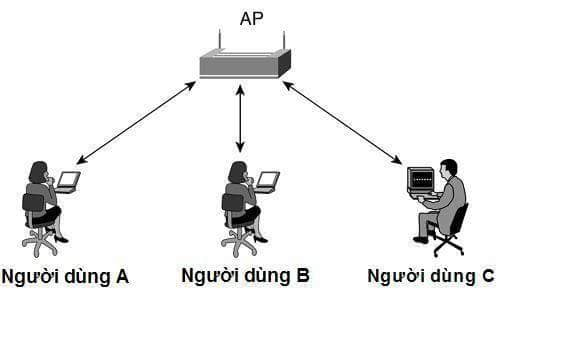
\includegraphics[width=0.75\textwidth]{BSS.jpg}
    \caption{Mô hình mạng cơ sở Basic Service Set (BSS)}
    \label{fig:bss}
\end{figure}

Đặc điểm của mô hình BSS:
\begin{itemize}
    \item Mỗi BSS được định danh bằng một mã định danh dịch vụ cơ bản BSSID (chính là địa chỉ MAC của card sóng vô tuyến trên AP).
    \item Toàn bộ các STA trong BSS chia sẻ chung một kênh tần số hoạt động của AP.
    \item Phạm vi phục vụ của BSS bị giới hạn bởi vùng phủ sóng vô tuyến (Basic Service Area -- BSA) của AP đơn lẻ.
\end{itemize}

\subsection{Mô hình mạng mở rộng (Extended Service Set -- ESS)}

Để đáp ứng nhu cầu phủ sóng trên diện tích lớn như toàn bộ khuôn viên trường đại học gồm nhiều khối nhà, chuẩn IEEE 802.11 định nghĩa mô hình Extended Service Set (ESS). Mô hình này kết hợp nhiều BSS lại với nhau thông qua một hệ thống phân phối chung (Distribution System -- DS), thường là mạng chuyển mạch có dây Ethernet tốc độ cao (Hình \ref{fig:ess}).

\begin{figure}[htbp]
    \centering
    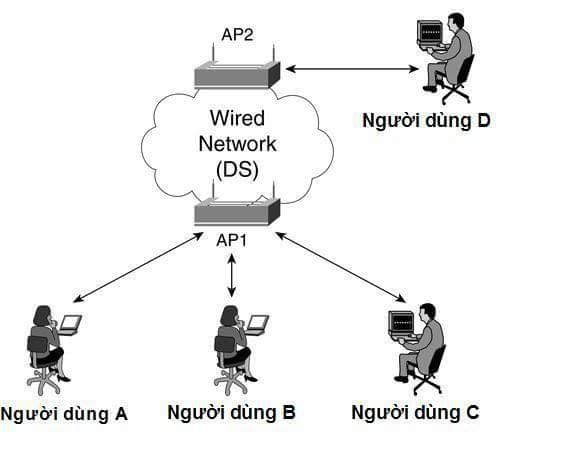
\includegraphics[width=0.85\textwidth]{ESS.jpg}
    \caption{Mô hình mạng mở rộng Extended Service Set (ESS)}
    \label{fig:ess}
\end{figure}

Đặc điểm nổi bật của ESS:
\begin{itemize}
    \item Tất cả các AP trong cùng một mạng ESS được cấu hình phát chung một tên mạng logic gọi là SSID (Service Set Identifier), cho phép người dùng nhìn thấy một hệ thống Wi-Fi đồng nhất duy nhất.
    \item Các AP đặt cạnh nhau được cấu hình trên các kênh tần số không chồng lấn để triệt tiêu nhiễu đồng kênh.
    \item Hỗ trợ cơ chế chuyển vùng (Roaming): Khi sinh viên cầm laptop hoặc điện thoại di chuyển từ tòa nhà này sang tòa nhà khác, thiết bị sẽ tự động ngắt kết nối với AP có tín hiệu yếu và liên kết sang AP có tín hiệu mạnh hơn mà vẫn duy trì liên tục phiên làm việc trên tầng ứng dụng.
\end{itemize}

\subsection{Mô hình mạng độc lập Ad-hoc (Independent BSS -- IBSS)}

Mô hình IBSS (còn gọi là mạng ngang hàng Ad-hoc) là mô hình không sử dụng Access Point trung tâm (Hình \ref{fig:ibss}). Các thiết bị di động trong cự ly gần tự động bắt tay và truyền nhận dữ liệu trực tiếp với nhau theo cơ chế Peer-to-Peer.

\begin{figure}[htbp]
    \centering
    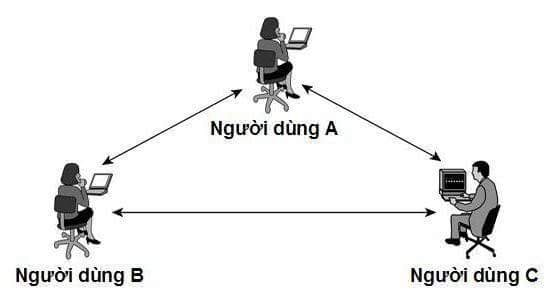
\includegraphics[width=0.75\textwidth]{IBSS.jpg}
    \caption{Mô hình mạng Ad-hoc (Independent BSS -- IBSS)}
    \label{fig:ibss}
\end{figure}

Mặc dù thiết lập nhanh và không tốn chi phí hạ tầng, mô hình IBSS không hỗ trợ quản trị tập trung, độ tin cậy thấp, khó triển khai bảo mật chặt chẽ và suy giảm hiệu năng nghiêm trọng khi số lượng máy trạm tăng. Do đó, mô hình này không được sử dụng trong các hệ thống mạng quy mô trường học hoặc doanh nghiệp.

\section{Cơ chế truy nhập kênh và kiểm soát xung đột trong WLAN}

\subsection{Cơ chế CSMA/CA}

Khác với mạng có dây Ethernet sử dụng cơ chế phát hiện va chạm CSMA/CD (Carrier Sense Multiple Access with Collision Detection), mạng không dây IEEE 802.11 bắt buộc phải sử dụng cơ chế tránh va chạm \textbf{CSMA/CA} (Carrier Sense Multiple Access with Collision Avoidance) \cite{kurose2021computer}. Nguyên nhân là do trong môi trường sóng vô tuyến, công suất phát tín hiệu tại anten của trạm phát lớn hơn hàng nghìn lần so với cường độ tín hiệu thu được từ các trạm khác, khiến máy phát không thể vừa phát sóng vừa lắng nghe để phát hiện va chạm trên đường truyền.

\begin{figure}[htbp]
    \centering
    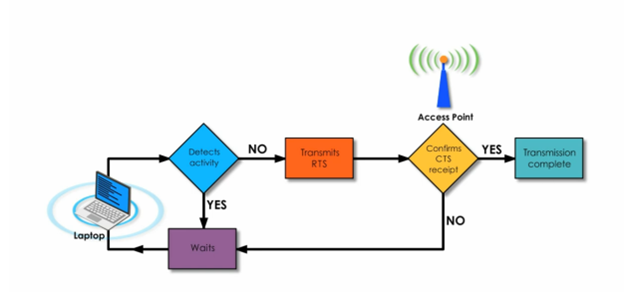
\includegraphics[width=0.9\textwidth]{CSMA-CA.png}
    \caption{Quy trình truyền dẫn dữ liệu sử dụng CSMA/CA và cơ chế bắt tay RTS/CTS}
    \label{fig:csma-ca}
\end{figure}

Quy trình hoạt động của thuật toán CSMA/CA (Hình \ref{fig:csma-ca}):
\begin{enumerate}
    \item \textbf{Cảm nhận sóng mang (Carrier Sense):} Trước khi gửi dữ liệu, thiết bị lắng nghe kênh truyền thông qua cảm nhận vật lý (Clear Channel Assessment -- CCA) và cảm nhận ảo dựa trên véc-tơ phân bổ mạng (Network Allocation Vector -- NAV).
    \item \textbf{Khoảng giãn cách khung (IFS) và Backoff:} Nếu kênh truyền rỗi trong khoảng thời gian phân tán DIFS (Distributed Inter-Frame Space), trạm sẽ tạo một giá trị thời gian chờ ngẫu nhiên gọi là khoảng lùi (Random Backoff). Thiết bị giảm dần giá trị bộ đếm lùi khi kênh rỗi; trạm nào giảm về 0 trước sẽ được quyền chiếm dụng kênh để phát tin.
    \item \textbf{Xác nhận truyền tin (ACK):} Sau khi nhận trọn vẹn khung dữ liệu Data Frame đúng mã kiểm tra CRC, bên nhận phải gửi lại một khung tin xác nhận ACK (Acknowledge) sau khoảng thời gian SIFS ngắn nhất. Nếu không nhận được ACK trong thời gian quy định, bên phát mặc định đã xảy ra va chạm và nhân đôi cửa sổ lùi (Binary Exponential Backoff) trước khi thử truyền lại.
\end{enumerate}

Bảng \ref{tab:csma_compare} tổng hợp các điểm khác biệt bản chất giữa hai cơ chế truy nhập kênh có dây và không dây:

\begin{table}[htbp]
\centering
\caption{So sánh cơ chế CSMA/CA (WLAN) và CSMA/CD (Ethernet)}
\label{tab:csma_compare}
\small
\begin{tabular}{lll}
\toprule
\textbf{Tiêu chí kỹ thuật} & \textbf{CSMA/CA (IEEE 802.11)} & \textbf{CSMA/CD (IEEE 802.3)} \\
\midrule
Môi trường truyền dẫn & Sóng vô tuyến không dây (Bán song công) & Cáp xoắn đôi / cáp quang có dây \\
Phương thức xử lý xung đột & Phòng ngừa và né tránh trước khi gửi & Phát hiện khi đang truyền và gửi tín hiệu Jamming \\
Khung tin xác nhận ACK & Bắt buộc ở lớp MAC & Không bắt buộc (xử lý ở tầng giao vận TCP) \\
Hiện tượng nút ẩn/nút lộ & Thường xuyên xảy ra & Không tồn tại \\
Hiệu suất kênh hữu ích & Thường đạt 50\% -- 60\% băng thông lý thuyết & Đạt $>90\%$ băng thông cáp \\
\bottomrule
\end{tabular}
\end{table}

\subsection{Hiện tượng nút ẩn và cơ chế bắt tay RTS/CTS}

Trong mạng không dây, hiện tượng \textbf{Nút ẩn (Hidden Node)} xảy ra khi hai máy trạm $STA_1$ và $STA_2$ cùng nằm trong tầm phủ sóng của một Access Point nhưng ở cách xa nhau ngoài tầm nghe thấy nhau. Khi cả hai trạm cùng cảm nhận kênh rỗi và đồng thời phát gói tin về phía AP, các luồng sóng sẽ va chạm dữ liệu tại anten của AP, gây hỏng gói tin.

Để giải quyết triệt để vấn đề này, chuẩn IEEE 802.11 tích hợp cơ chế bắt tay trước khi truyền:
\begin{itemize}
    \item Trạm gửi gói tin ngắn \textbf{RTS (Request to Send)} chứa thông tin thời gian cần chiếm dụng kênh.
    \item AP phản hồi bằng khung \textbf{CTS (Clear to Send)} broadcast cho toàn bộ các trạm xung quanh biết.
    \item Tất cả các trạm khác nghe được CTS sẽ thiết lập bộ đếm ảo NAV và tạm ngừng truyền cho đến khi trạm gửi hoàn tất giao dịch.
\end{itemize}

\section{Băng tần vô tuyến, phân bổ kênh và can nhiễu trong WLAN}

\subsection{Các băng tần vô tuyến phổ biến}

Mạng Wi-Fi hoạt động trên các băng tần vô tuyến thuộc nhóm băng tần công nghiệp, khoa học và y tế (ISM) không cần cấp phép (Unlicensed Bands):
\begin{itemize}
    \item \textbf{Băng tần 2.4 GHz (2.400 -- 2.4835 GHz):} Băng tần truyền thống, bước sóng dài nên có khả năng xuyên vật cản (bê tông, gạch đá) rất tốt và phạm vi phủ sóng rộng. Tuy nhiên, băng thông tổng chỉ khoảng 83.5 MHz, chỉ chứa được tối đa 3 kênh độc lập không chồng lấn. Đồng thời, dải tần này bị can nhiễu nặng nề bởi sóng Bluetooth, lò vi sóng và các thiết bị ngoại lai.
    \item \textbf{Băng tần 5 GHz (5.150 -- 5.850 GHz):} Băng thông rộng lớn lên tới hơn 500 MHz, cung cấp tới 24 kênh không chồng lấn có độ rộng 20 MHz. Tốc độ truyền tải rất cao, ít can nhiễu. Nhược điểm là bước sóng ngắn nên khả năng đâm xuyên tường kém hơn đáng kể so với 2.4 GHz.
    \item \textbf{Băng tần 6 GHz (5.925 -- 7.125 GHz):} Được áp dụng trong chuẩn Wi-Fi 6E và Wi-Fi 7, mở ra thêm 1.200 MHz phổ tần sạch hoàn toàn, hỗ trợ tới 14 kênh rộng 80 MHz và 7 kênh siêu rộng 160 MHz, chuyên biệt cho các tác vụ đòi hỏi thông lượng gigabit và độ trễ cực thấp.
\end{itemize}

\subsection{Quy hoạch kênh không chồng lấn tại dải 2.4 GHz}

Tại dải tần 2.4 GHz, phổ sóng được phân thành 11 kênh (tại Bắc Mỹ) hoặc 13 kênh (tại Châu Á và Việt Nam). Khoảng cách giữa các tần số trung tâm chỉ là 5 MHz trong khi độ rộng của mỗi kênh Wi-Fi tiêu chuẩn là 20 MHz hoặc 22 MHz. Do đó, các kênh nằm kề nhau sẽ có dải tần chồng lấn lên nhau.

Trong toàn bộ dải 2.4 GHz, chỉ có đúng \textbf{3 kênh duy nhất hoàn toàn không chồng lấn} là kênh \textbf{1, 6 và 11}. Khi thiết kế mạng Wi-Fi trường học, nguyên tắc quy hoạch cơ bản là phân bổ xen kẽ các kênh 1, 6, 11 giữa các AP kề nhau trên cùng một mặt sàn và giữa các tầng nhà, triệt tiêu tối đa hiện tượng can nhiễu đồng kênh (Co-channel Interference).

\section{Tiến trình phát triển các thế hệ chuẩn Wi-Fi và Công nghệ Wi-Fi 6}

Bảng \ref{tab:wifi_evolution} tóm tắt tiến trình phát triển của các thế hệ chuẩn IEEE 802.11 từ khởi thủy đến nay:

\begin{table}[htbp]
\centering
\caption{Tổng hợp so sánh tiến hóa các thế hệ chuẩn mạng không dây IEEE 802.11}
\label{tab:wifi_evolution}
\small
\begin{tabular}{lcccccc}
\toprule
\textbf{Chuẩn} & \textbf{Tên gọi} & \textbf{Năm ban hành} & \textbf{Băng tần} & \textbf{Kênh rộng} & \textbf{Tốc độ tối đa} & \textbf{Kỹ thuật điều chế} \\
\midrule
802.11b & Wi-Fi 1 & 1999 & 2.4 GHz & 20 MHz & 11 Mbps & DSSS \\
802.11a & Wi-Fi 2 & 1999 & 5 GHz & 20 MHz & 54 Mbps & OFDM \\
802.11g & Wi-Fi 3 & 2003 & 2.4 GHz & 20 MHz & 54 Mbps & OFDM \\
802.11n & Wi-Fi 4 & 2009 & 2.4 / 5 GHz & 20, 40 MHz & 600 Mbps & MIMO, 64-QAM \\
802.11ac & Wi-Fi 5 & 2013 & 5 GHz & 20, 40, 80, 160 & 6.9 Gbps & MU-MIMO, 256-QAM \\
802.11ax & \textbf{Wi-Fi 6} & \textbf{2021} & \textbf{2.4 / 5 / 6 GHz} & \textbf{20, 40, 80, 160} & \textbf{9.6 Gbps} & \textbf{OFDMA, 1024-QAM} \\
802.11be & Wi-Fi 7 & 2024+ & 2.4 / 5 / 6 GHz & Đến 320 MHz & 46 Gbps & MLO, 4096-QAM \\
\bottomrule
\end{tabular}
\end{table}

\subsection{Các công nghệ đột phá của chuẩn Wi-Fi 6 (IEEE 802.11ax)}

Chuẩn IEEE 802.11ax (Wi-Fi 6) được thiết kế đặc thù không chỉ nhằm tăng tốc độ đỉnh (Peak Throughput) mà mục tiêu trọng tâm là cải thiện hiệu quả sử dụng phổ tần trong môi trường có mật độ thiết bị cực cao (High Density -- HD) như giảng đường đại học \cite{khorov2019tutorial}:

\begin{enumerate}
    \item \textbf{Kỹ thuật đa truy nhập phân chia theo tần số trực giao (OFDMA):} Đây là công nghệ cốt lõi mượn từ mạng di động 4G/5G. Thay vì cho phép một người dùng duy nhất chiếm dụng toàn bộ kênh truyền 20 MHz hoặc 40 MHz tại một thời điểm, OFDMA chia nhỏ kênh sóng thành các khối tần số con gọi là \textbf{Resource Units (RU)}. Một khung truyền vô tuyến có thể phục vụ đồng thời lên tới hàng chục người dùng khác nhau trong cùng một thời điểm, triệt tiêu tình trạng nghẽn hàng đợi đối với các gói tin nhỏ.
    \item \textbf{Công nghệ MU-MIMO đa người dùng 8x8 cả Uplink và Downlink:} Cho phép AP phát và thu đồng thời nhiều luồng dữ liệu không phụ thuộc tới các nhóm thiết bị khác nhau, nâng gấp đôi hiệu suất truyền dẫn so với Wi-Fi 5 vốn chỉ hỗ trợ MU-MIMO ở chiều Downlink.
    \item \textbf{Kỹ thuật tô màu định danh bản tin (BSS Coloring):} Trong chuẩn cũ, khi phát hiện bất kỳ tín hiệu nào cùng tần số (dù phát ra từ phòng học kế bên), máy trạm phải hoãn phiên truyền. Wi-Fi 6 bổ sung trường mã màu 6-bit vào phần đầu khung tin. Khi máy trạm nhận thấy sóng mang có mã màu khác với BSS của mình, nó nhận diện đây là tín hiệu xuyên phòng vô hại và vẫn tiếp tục thực hiện phát dữ liệu, giảm thiểu hơn 60\% thời gian chờ đợi vô ích do can nhiễu đồng kênh.
\end{enumerate}

\section{Kiến trúc quản lý mạng không dây tập trung (Wireless LAN Controller)}

Trong môi trường mạng doanh nghiệp và trường đại học (Enterprise Campus Network), mô hình quản trị truyền thống sử dụng các AP độc lập (Autonomous AP) bộc lộ nhược điểm chí mạng: mỗi AP phải được cấu hình riêng rẽ, không có khả năng tự động điều phối tần số và không thể thực hiện chuyển vùng mượt mà \cite{cisco2021wlan}.

Kiến trúc mạng không dây hiện đại chuyển dịch hoàn toàn sang mô hình \textbf{AP hạng nhẹ kết hợp Bộ điều khiển trung tâm (Lightweight AP + WLC)} dựa trên nguyên lý phân tách lớp điều khiển MAC (Split-MAC Architecture):

\begin{itemize}
    \item \textbf{Phần MAC cục bộ trên AP (Local MAC):} AP chỉ đảm nhận các tác vụ thời gian thực lớp vật lý như phát sóng RF, mã hóa/giải mã phần cứng, gửi nhận khung tin Beacon và ACK.
    \item \textbf{Phần MAC tập trung trên WLC (Centralized MAC):} Bộ điều khiển trung tâm WLC đảm nhận việc xử lý xác thực danh tính người dùng (802.1X/RADIUS), chính sách gán VLAN, lọc địa chỉ MAC, định tuyến lưu lượng và quản trị roaming.
    \item \textbf{Đường hầm CAPWAP (Control and Provisioning of Wireless Access Points):} Toàn bộ lưu lượng điều khiển và dữ liệu người dùng giữa AP và WLC được đóng gói và mã hóa thông qua giao thức đường hầm CAPWAP (cổng UDP 5246 cho luồng Control và 5247 cho luồng Data).
    \item \textbf{Cơ chế Quản lý tài nguyên vô tuyến tự động (Radio Resource Management -- RRM):} WLC liên tục nhận thông tin đo kiểm môi trường RF từ các AP gửi về để tự động kích hoạt thuật toán gán kênh động (Dynamic Channel Assignment -- DCA) và kiểm soát công suất phát (Transmit Power Control -- TPC), đảm bảo hệ thống luôn tự lành (\textit{Self-healing}) khi có một AP bị sự cố phần cứng.
\end{itemize}

\section{Cơ chế chuyển vùng nhanh (Fast Roaming: IEEE 802.11r/k/v)}

Chuyển vùng (Roaming) là quá trình thiết bị di động ngắt kết nối với AP hiện tại và thiết lập liên kết mới với một AP lân cận có cường độ sóng mạnh hơn. Trong các mạng Wi-Fi bảo mật truyền thống (WPA2-Enterprise), quá trình roaming đòi hỏi trao đổi lại trọn vẹn quy trình bắt tay 802.1X với máy chủ RADIUS, gây độ trễ từ 500 ms đến 2.000 ms, dẫn đến rớt kết nối cuộc gọi thoại, video hoặc ứng dụng thi trực tuyến.

Hệ thống mạng không dây hiện đại giải quyết bài toán này thông qua bộ ba tiêu chuẩn:
\begin{itemize}
    \item \textbf{IEEE 802.11r (Fast BSS Transition -- FT):} Cho phép lưu sẵn các khóa mật mã xác thực giữa WLC và các AP mục tiêu lân cận. Khi thiết bị di chuyển, quá trình bắt tay được rút gọn chỉ còn 4 gói tin trao đổi cục bộ, giảm độ trễ chuyển vùng xuống dưới \textbf{50 ms}.
    \item \textbf{IEEE 802.11k (Radio Resource Measurement):} AP cung cấp cho máy trạm danh sách báo cáo các AP lân cận tối ưu (Neighbor Report), giúp thiết bị không phải quét toàn bộ các kênh tần số, tiết kiệm pin và đẩy nhanh tốc độ dò sóng.
    \item \textbf{IEEE 802.11v (BSS Transition Management):} Cho phép WLC chủ động gửi lệnh điều hướng thiết bị di động chuyển sang AP khác gần hơn khi nhận thấy cường độ sóng của AP hiện tại suy yếu, giải quyết triệt để vấn nạn thiết bị ``bám dính'' trạm phát sóng ở xa (\textit{Sticky Client}).
\end{itemize}

\section{Tiểu kết Chương 1}

Chương 1 đã hệ thống hóa toàn diện các nền tảng lý thuyết cốt lõi về mạng cục bộ không dây WLAN:
\begin{enumerate}
    \item Phân tích bản chất các mô hình BSS, ESS và cơ chế truy nhập kênh tránh va chạm CSMA/CA kết hợp bắt tay RTS/CTS.
    \item Làm rõ đặc thù các băng tần 2.4 GHz, 5 GHz và quy tắc phân bổ 3 kênh không chồng lấn (1, 6, 11).
    \item Đánh giá sự vượt trội của thế hệ Wi-Fi 6 với các công nghệ then chốt OFDMA, MU-MIMO và BSS Coloring trong việc giải quyết bài toán môi trường mật độ cao.
    \item Khẳng định tính tất yếu của mô hình quản trị tập trung WLC dựa trên giao thức CAPWAP và bộ giao thức chuyển vùng nhanh IEEE 802.11r/k/v.
\end{enumerate}

Những nội dung khoa học này là cơ sở vững chắc để tiến hành khảo sát thực địa, chẩn đoán điểm nghẽn tại Trường Đại học Đồng Tháp ở Chương 2 và xây dựng kiến trúc thiết kế tối ưu ở Chương 3.


\chapter{Khảo sát và đánh giá hiện trạng mạng không dây tại Trường Đại học Đồng Tháp}
\label{chap:hien-trang}

Trên cơ sở nền tảng lý thuyết đã được trình bày ở Chương \ref{chap:ly-thuyet}, Chương 2 sẽ đi sâu vào việc khảo sát thực tế, đo kiểm và đánh giá toàn diện hiện trạng hệ thống mạng không dây tại Trường Đại học Đồng Tháp. Nội dung chương này tập trung làm rõ sơ đồ phân bố hạ tầng, đánh giá năng lực chịu tải của thiết bị điều khiển trung tâm (WLC), phân tích dữ liệu quét sóng Wi-Fi thực tế tại các phân khu trọng điểm (Tòa A1, Tòa B3, Tòa B5). Qua đó, chương này sẽ xác định các nguyên nhân ảnh hưởng đến chất lượng mạng, tình trạng can nhiễu đồng kênh và rủi ro từ các thiết bị phát sóng ngoại lai, làm cơ sở cho việc xây dựng giải pháp tối ưu ở Chương \ref{chap:giai-phap}.

\section{Giới thiệu tổng quan hệ thống mạng không dây tại Đại học Đồng Tháp}

Hệ thống mạng không dây tại Trường Đại học Đồng Tháp được triển khai nhằm phục vụ nhu cầu truy cập Internet cho cán bộ, giảng viên và sinh viên trong quá trình học tập, giảng dạy và nghiên cứu khoa học. Wi-Fi hiện diện ở hầu hết các khu vực như giảng đường, phòng thực hành, phòng làm việc hành chính, thư viện và các khu vực sinh hoạt chung trong khuôn viên nhà trường.

Các thiết bị Access Point (AP) được lắp đặt rải rác tại nhiều tòa nhà như A1, A2, A7, A8, A9, C1, C2, H1, H2, H3, B1, B2, B3, B4, B5, B6, Thư viện, Giảng đường 1... và được kết nối về hệ thống mạng lõi nội bộ để cung cấp dịch vụ Internet cho người dùng \cite{dthu2026hientrang}.

\subsection{Sơ đồ tổng thể toàn trường}

Sơ đồ tổng quan của Trường Đại học Đồng Tháp được thể hiện chi tiết tại Hình \ref{fig:tong-the-truong}, bao gồm các phân khu chức năng chính:
\begin{itemize}
    \item \textbf{Khu học tập và giảng đường:} Gồm các khối nhà B1, B2, B3, A1, H1, H2, H3, C1, C2 phục vụ giảng dạy lý thuyết, phòng máy vi tính và các phòng thí nghiệm chuyên sâu.
    \item \textbf{Thư viện Học liệu Lê Vũ Hùng:} Đặt ở vị trí trung tâm khuôn viên, là không gian tự học và tra cứu thông tin số tập trung đông đảo sinh viên.
    \item \textbf{Khu thể thao và không gian chung:} Sân vận động, nhà thi đấu, hồ bơi, căn tin mở B5 và quảng trường A3.
    \item \textbf{Khu ký túc xá và sinh hoạt sinh viên:} Khối ký túc xá B6 và các nhà xe sinh viên.
\end{itemize}

\begin{figure}[htbp]
    \centering
    
\includegraphics[width=0.92\textwidth]{dthu_fig-001.png}
    \caption{Sơ đồ tổng thể khuôn viên Trường Đại học Đồng Tháp}
    \label{fig:tong-the-truong}
\end{figure}

Đặc thù khuôn viên rộng lớn và phân tán thành nhiều khối công trình kiến trúc riêng biệt đặt ra thách thức rất lớn trong việc phủ sóng Wi-Fi liên tục, đòi hỏi phải có chiến lược quy hoạch thiết bị Access Point phù hợp với đặc tính vật lý và mật độ người dùng của từng khu vực.

\subsection{Sơ đồ mạng tổng thể của Trường Đại học Đồng Tháp}

Để hiểu rõ phương thức vận hành và phân bổ luồng dữ liệu của toàn bộ hệ thống, quá trình khảo sát đã thu thập và hệ thống hóa cấu trúc mạng logic thực tế của Nhà trường như minh họa tại Hình \ref{fig:so-do-mang-tong-the}.

\begin{figure}[htbp]
    \centering
    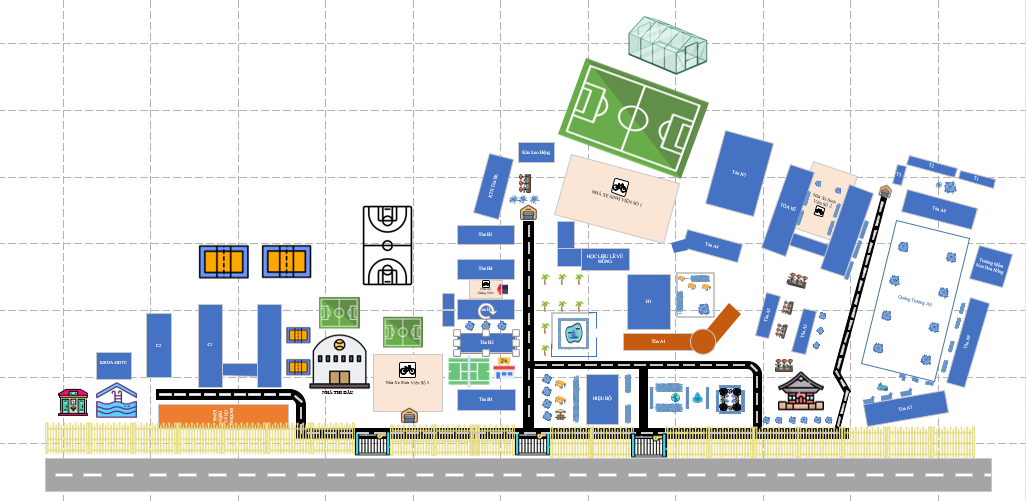
\includegraphics[width=0.95\textwidth]{dthu_fig-002.png}
    \caption{Sơ đồ mạng tổng thể tại Trường Đại học Đồng Tháp}
    \label{fig:so-do-mang-tong-the}
\end{figure}

Hệ thống được tổ chức theo mô hình mạng phân cấp truyền thống:
\begin{itemize}
    \item \textbf{Lớp Lõi (Core Layer):} Bộ định tuyến trung tâm và hệ thống máy chủ đóng vai trò điều phối toàn bộ lưu lượng dữ liệu nội bộ và kết nối ra mạng Internet qua các nhà cung cấp dịch vụ viễn thông (ISP).
    \item \textbf{Lớp Phân phối (Distribution Layer):} Hạ tầng được phân hoạch thành các nhánh mạng cục bộ ảo (VLAN) độc lập tương ứng với các đơn vị: Khối Hành chính, Khối Giảng đường, Khối Khoa chuyên môn và Khối Ký túc xá.
    \item \textbf{Lớp Truy cập (Access Layer) và WLAN:} Tại các phân khu, tín hiệu từ Switch phân phối được truyền trực tiếp tới các thiết bị Switch Access và các Access Point (AP) để phát sóng vô tuyến.
\end{itemize}

\subsection{Mô hình mô phỏng hệ thống trên Cisco Packet Tracer}

Nhằm phục vụ cho công tác phân tích chuyên sâu các điểm nghẽn và làm cơ sở thử nghiệm các giải pháp tối ưu hóa, toàn bộ kiến trúc mạng thực tế ở trên đã được số hóa và mô phỏng trên phần mềm Cisco Packet Tracer (Hình \ref{fig:mo-phong-cisco}).

\begin{figure}[htbp]
    \centering
    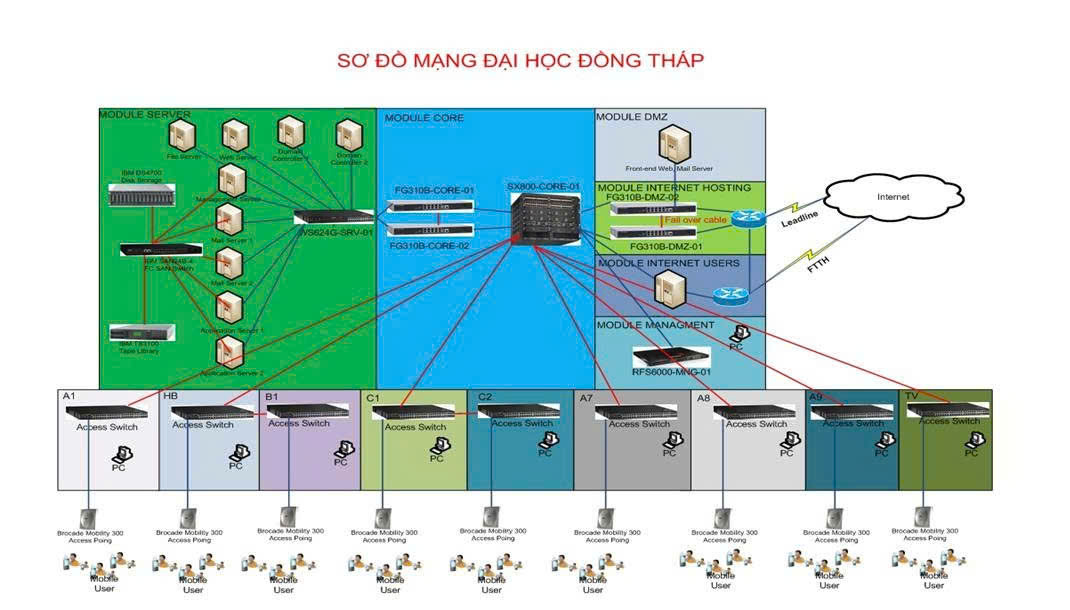
\includegraphics[width=0.95\textwidth]{dthu_fig-003.png}
    \caption{Mô hình mô phỏng hạ tầng mạng trên Cisco Packet Tracer}
    \label{fig:mo-phong-cisco}
\end{figure}

Việc sử dụng Packet Tracer cho phép thiết lập chính xác các thông số định tuyến, cấu trúc VLAN và mô phỏng các kịch bản lưu lượng truy cập cao trong giờ cao điểm, từ đó đánh giá được độ trễ và tỷ lệ rớt gói trước khi đề xuất giải pháp thiết kế mới.

\section{Khảo sát hạ tầng thiết bị và vị trí lắp đặt Access Point}

\subsection{Thiết bị điều khiển trung tâm (Wireless Switch)}

Hệ thống mạng không dây của Nhà trường hiện đang được quản lý thông qua thiết bị điều khiển \textbf{Motorola RFS6000 Wireless Switch} đặt tại phòng máy chủ trung tâm. Thông số kỹ thuật danh định của thiết bị:
\begin{itemize}
    \item Giao diện vật lý: Hỗ trợ 8 cổng kết nối Gigabit Ethernet (10/100/1000 Mbps).
    \item Khả năng quản lý: Hỗ trợ quản lý độc lập 48 Access Point (có thể mở rộng lên 256 AP khi ghép cụm cluster).
    \item Năng lực chịu tải (Capacity): Cấp phép truy cập đồng thời tối đa cho \textbf{2.000 thiết bị người dùng} (Concurrent Users).
    \item Băng thông chuyển mạch (Switching Capacity): 8 Gbps.
\end{itemize}

\textbf{Đánh giá mức độ đáp ứng và phân tích điểm nghẽn:}
Với quy mô toàn trường hơn 15.000 sinh viên, lưu lượng kết nối Wi-Fi thực tế biến động rất mạnh theo các khung giờ học tập (Bảng \ref{tab:tai_luong_wlc}).

\begin{table}[htbp]
\centering
\caption{Thống kê tải lượng thiết bị kết nối đồng thời trong ngày}
\label{tab:tai_luong_wlc}
\begin{tabular}{lcl}
\toprule
\textbf{Thời điểm khảo sát} & \textbf{Số lượng thiết bị kết nối} & \textbf{Trạng thái hệ thống WLC} \\
\midrule
07h00 -- 08h00 (Đầu giờ sáng) & Khoảng 850 thiết bị & Hoạt động ổn định, cấp IP nhanh chóng \\
09h30 -- 10h30 (Cao điểm sáng) & Khoảng 2.150 thiết bị & Vượt ngưỡng 2.000, trễ nhịp cấp phát IP \\
14h00 -- 15h30 (Cao điểm chiều) & Khoảng 2.300 thiết bị & Treo DHCP, từ chối cấp IP cho máy mới \\
\bottomrule
\end{tabular}
\end{table}

Khi tổng số thiết bị kết nối vượt ngưỡng 2.000, bộ điều khiển rơi vào trạng thái cạn kiệt tài nguyên cấp phát (DHCP Exhaustion) và quá tải năng lực xử lý. Đây là nguyên nhân trực tiếp giải thích hiện tượng sinh viên thấy điện thoại báo sóng Wi-Fi đầy vạch nhưng không thể nhận được địa chỉ IP để truy cập mạng.

\subsection{Khảo sát vị trí lắp đặt Access Point tại các khối công trình}

Quá trình khảo sát đã lập bản đồ định vị các trạm phát sóng AP trên bản vẽ mặt bằng các tòa nhà:

\subsubsection{Khối giảng đường mật độ cao (Tòa C2, Tòa A1)}
Tại các tòa nhà phục vụ học lý thuyết đại trà (Tòa C2 -- Hình \ref{fig:ap-c2} và Tòa A1 -- Hình \ref{fig:ap-a1}), các AP được lắp dọc theo trục hành lang chính với cự ly 12m -- 15m. Mật độ lắp đặt dày đặc nhằm chia nhỏ tải lượng thiết bị kết nối, tuy nhiên cách bố trí này đòi hỏi quy hoạch kênh tần số rất khắt khe để tránh giao thoa sóng xuyên tầng.

\begin{figure}[htbp]
    \centering
    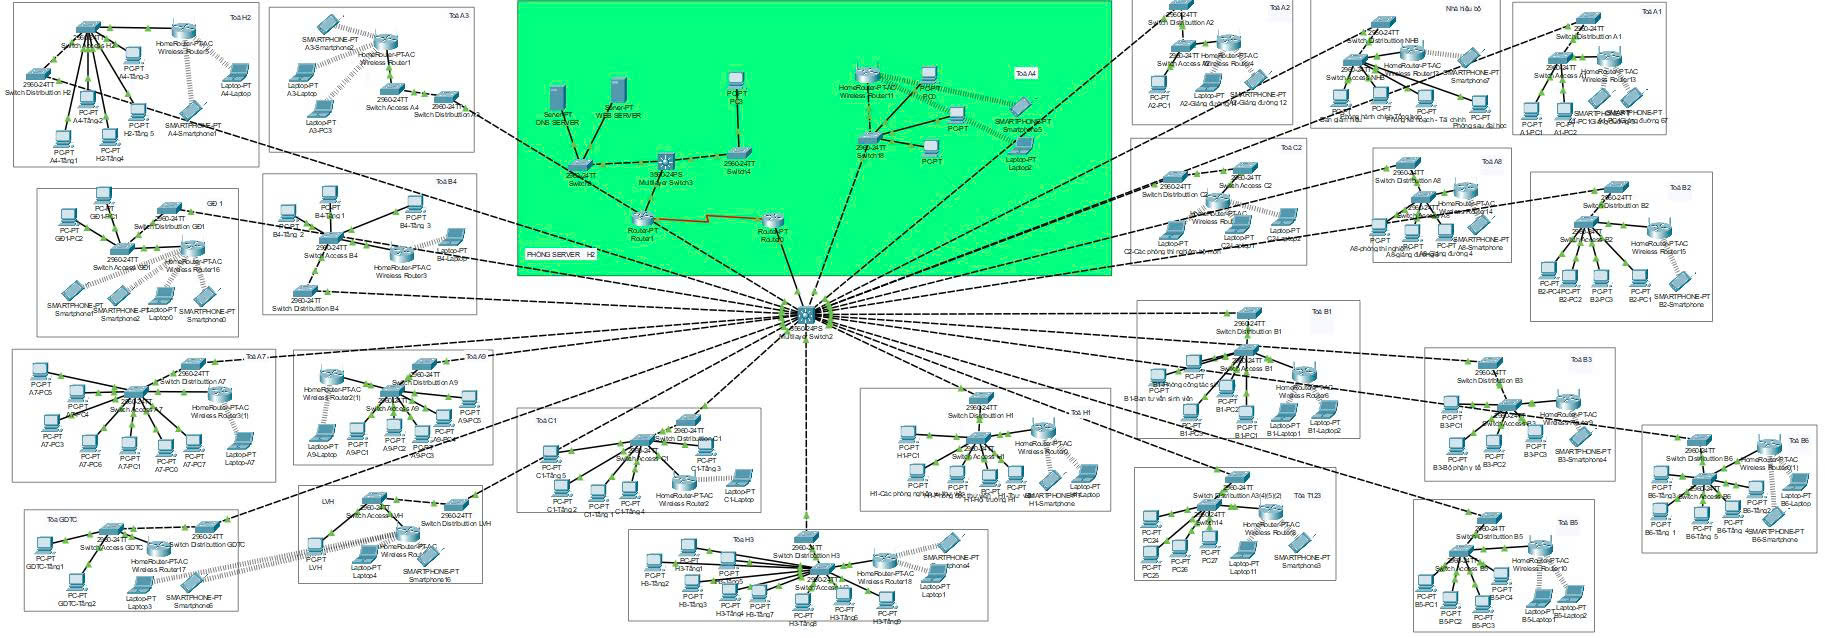
\includegraphics[width=0.88\textwidth]{dthu_fig-004.png}
    \caption{Sơ đồ vị trí lắp đặt Access Point tại Tòa C2}
    \label{fig:ap-c2}
\end{figure}

\begin{figure}[htbp]
    \centering
    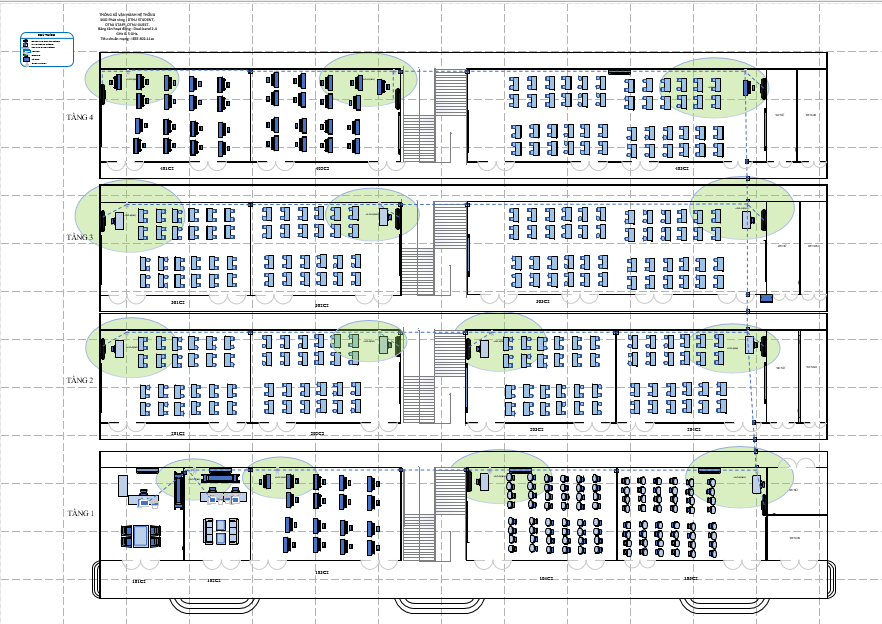
\includegraphics[width=0.88\textwidth]{dthu_fig-005.png}
    \caption{Sơ đồ vị trí lắp đặt Access Point tại Tòa A1}
    \label{fig:ap-a1}
\end{figure}

\subsubsection{Khối phòng thực hành và nghiên cứu (Tòa A2, A7, A8, A9, A4)}
Các tòa nhà này chủ yếu phục vụ các phòng máy tính và phòng thí nghiệm (Hình \ref{fig:ap-a2} đến Hình \ref{fig:ap-a4}). Phần lớn máy tính cố định sử dụng cáp LAN, do đó các AP Wi-Fi được bố trí với mật độ vừa phải tại hành lang và phòng hội đồng, ưu tiên vùng phủ sóng băng tần 5 GHz.

\begin{figure}[htbp]
    \centering
    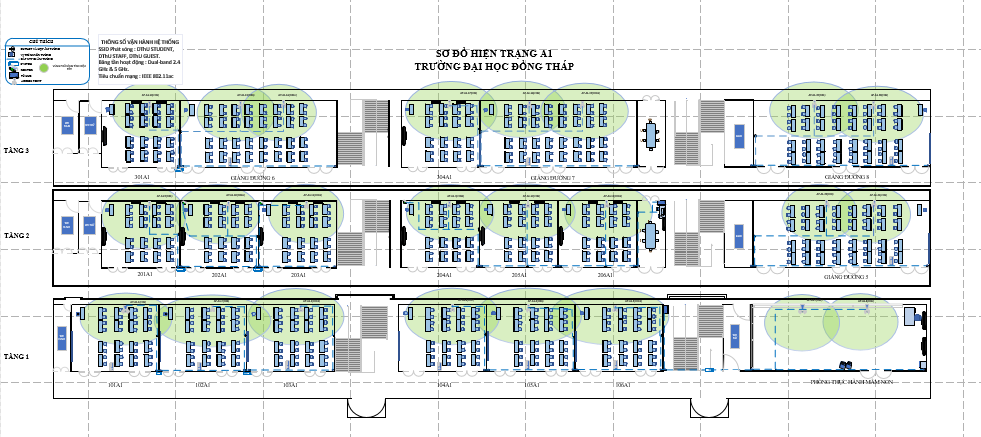
\includegraphics[width=0.85\textwidth]{dthu_fig-006.png}
    \caption{Sơ đồ vị trí lắp đặt Access Point tại Tòa A2}
    \label{fig:ap-a2}
\end{figure}

\begin{figure}[htbp]
    \centering
    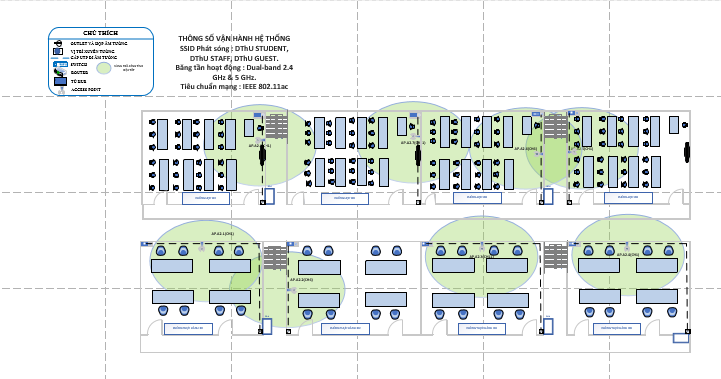
\includegraphics[width=0.85\textwidth]{dthu_fig-007.png}
    \caption{Sơ đồ vị trí lắp đặt Access Point tại Tòa A7}
    \label{fig:ap-a7}
\end{figure}

\begin{figure}[htbp]
    \centering
    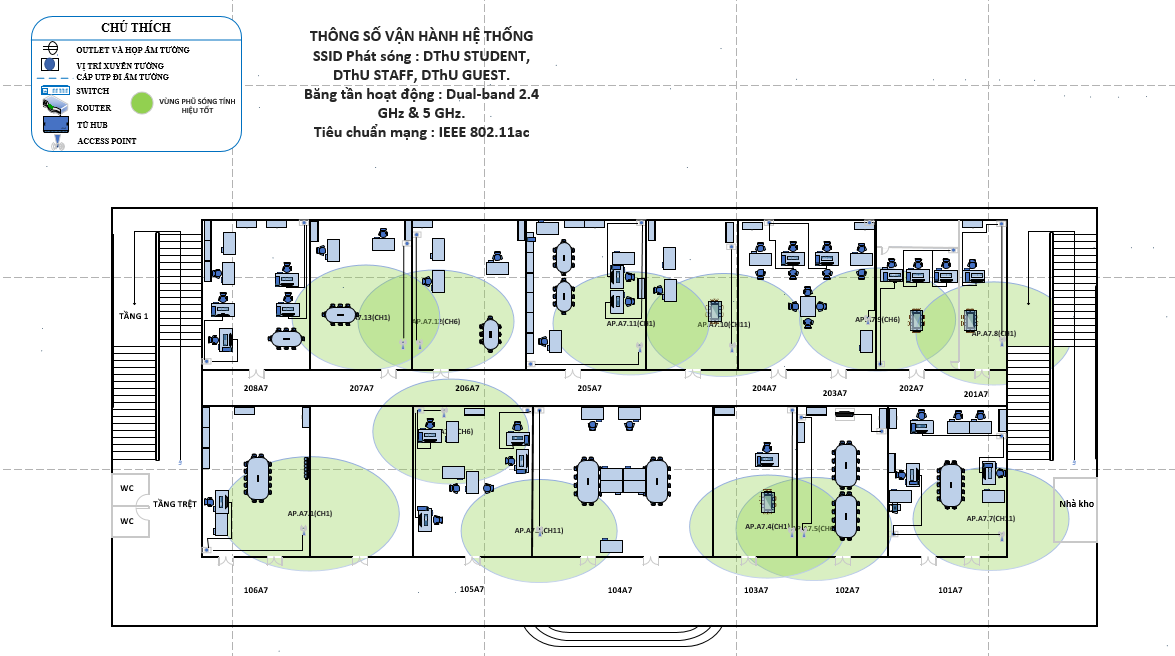
\includegraphics[width=0.85\textwidth]{dthu_fig-008.png}
    \caption{Sơ đồ vị trí lắp đặt Access Point tại Tòa A8}
    \label{fig:ap-a8}
\end{figure}

\begin{figure}[htbp]
    \centering
    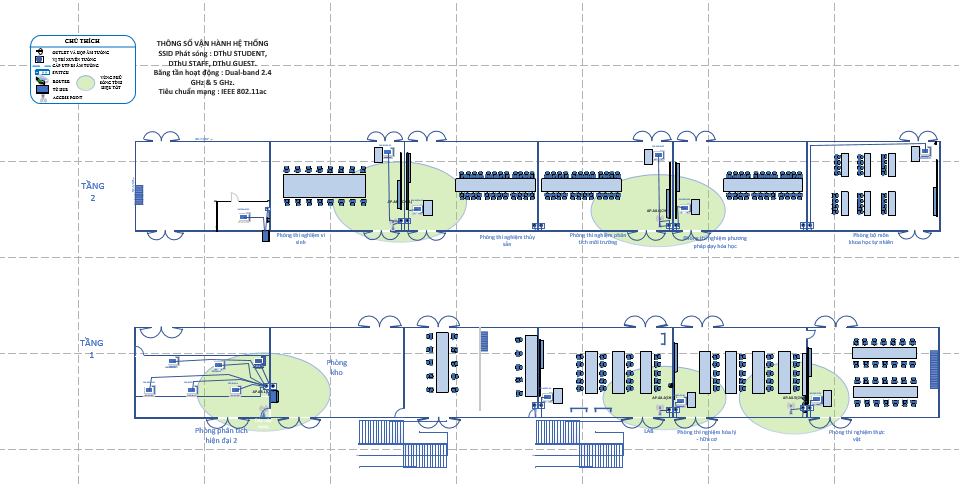
\includegraphics[width=0.85\textwidth]{dthu_fig-009.png}
    \caption{Sơ đồ vị trí lắp đặt Access Point tại Tòa A9}
    \label{fig:ap-a9}
\end{figure}

\begin{figure}[htbp]
    \centering
    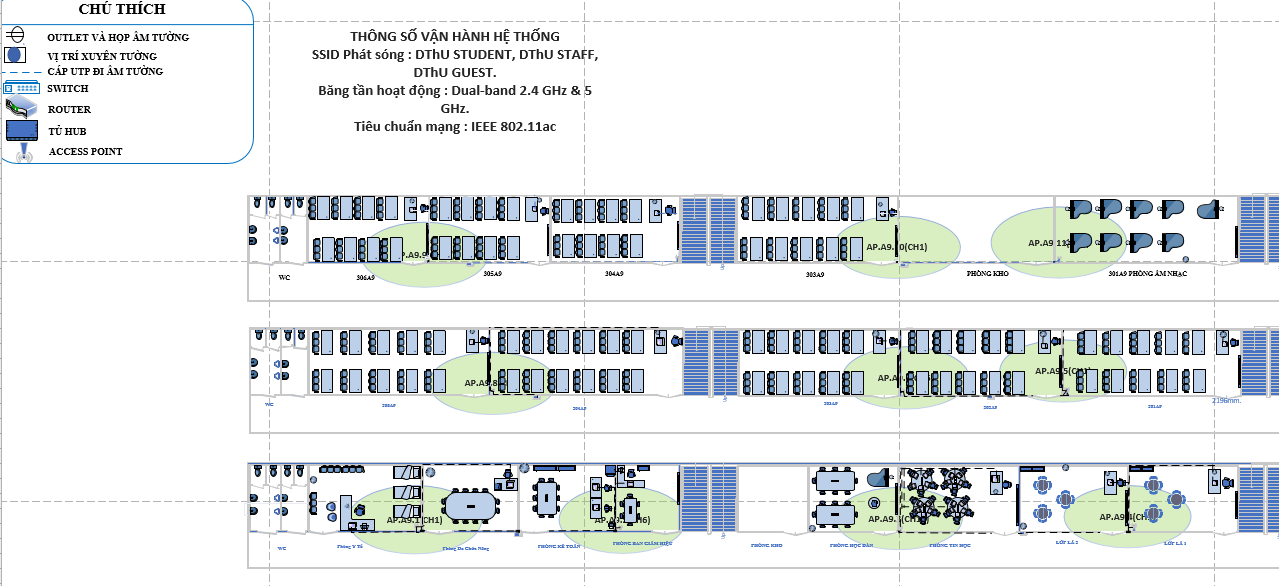
\includegraphics[width=0.85\textwidth]{dthu_fig-010.png}
    \caption{Sơ đồ vị trí lắp đặt Access Point tại Tòa A4}
    \label{fig:ap-a4}
\end{figure}

\subsubsection{Khối nhà Hành chính và Văn phòng (Tòa B1, B2, B3)}
Khối nhà hành chính (Hình \ref{fig:ap-b1} đến Hình \ref{fig:ap-b3}) có đặc điểm nhiều phòng làm việc ngăn cách bởi tường bê tông kiên cố. Sóng vô tuyến từ hành lang suy hao mạnh khi đâm xuyên vào các góc khuất, tạo ra vùng lõm sóng.

\begin{figure}[htbp]
    \centering
    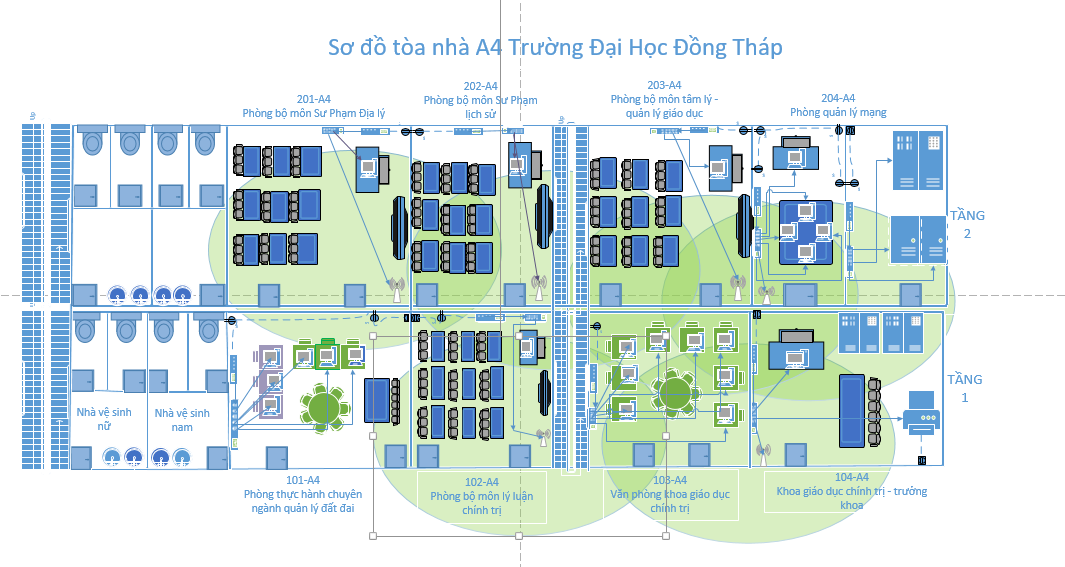
\includegraphics[width=0.85\textwidth]{dthu_fig-011.png}
    \caption{Sơ đồ vị trí lắp đặt Access Point tại Tòa B1}
    \label{fig:ap-b1}
\end{figure}

\begin{figure}[htbp]
    \centering
    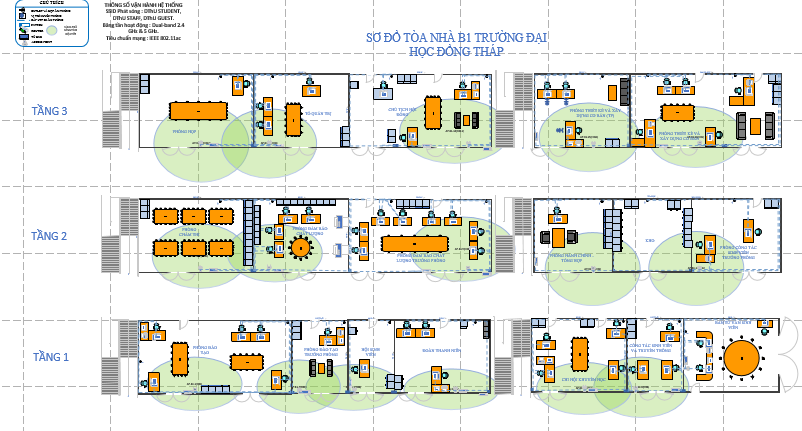
\includegraphics[width=0.85\textwidth]{dthu_fig-012.png}
    \caption{Sơ đồ vị trí lắp đặt Access Point tại Tòa B2}
    \label{fig:ap-b2}
\end{figure}

\begin{figure}[htbp]
    \centering
    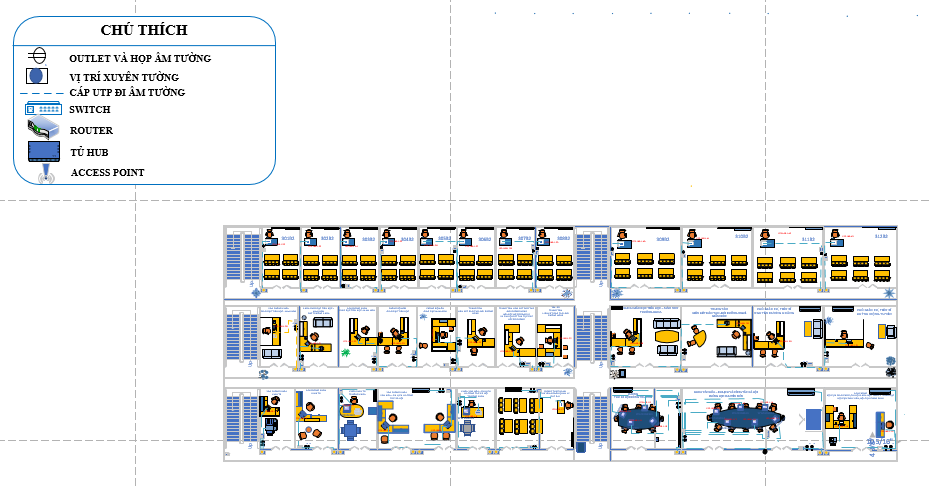
\includegraphics[width=0.85\textwidth]{dthu_fig-013.png}
    \caption{Sơ đồ vị trí lắp đặt Access Point tại Tòa B3}
    \label{fig:ap-b3}
\end{figure}

\subsubsection{Khối không gian mở Căn tin B5 và Ký túc xá B6}
Tòa B5 (Hình \ref{fig:ap-b5}) là không gian căn tin mở hoàn toàn, tập trung hàng trăm sinh viên vào giờ nghỉ giải lao. AP được treo cao trên trần để phủ sóng rộng, song việc thiếu vách ngăn khiến sóng các AP tràn lấn mạnh mẽ. Trong khi đó, Ký túc xá B6 (Hình \ref{fig:ap-b6}) bố trí AP dọc hành lang nhằm đâm xuyên vào các phòng nội trú.

\begin{figure}[htbp]
    \centering
    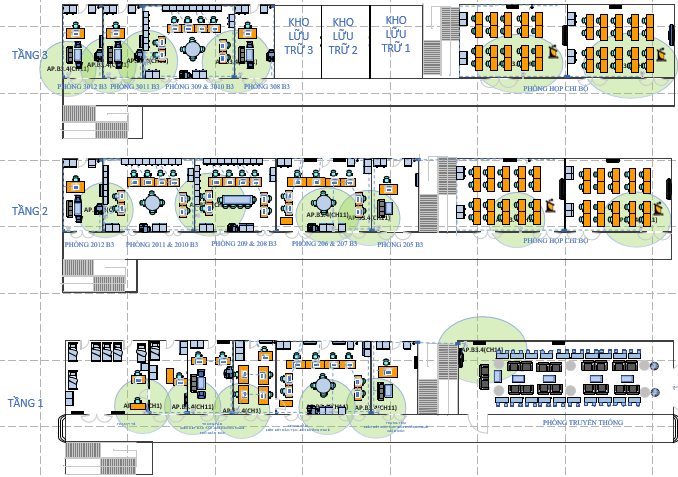
\includegraphics[width=0.82\textwidth]{dthu_fig-014.png}
    \caption{Sơ đồ vị trí lắp đặt Access Point tại Tòa B5 (Căn tin)}
    \label{fig:ap-b5}
\end{figure}

\begin{figure}[htbp]
    \centering
    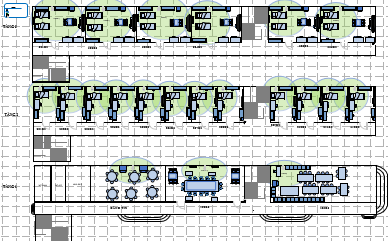
\includegraphics[width=0.82\textwidth]{dthu_fig-015.png}
    \caption{Sơ đồ vị trí lắp đặt Access Point tại KTX B6}
    \label{fig:ap-b6}
\end{figure}

\section{Phân tích vùng phủ sóng và can nhiễu vô tuyến thực tế}

Để kiểm chứng định lượng các nhược điểm vật lý của hệ thống, tác giả đã sử dụng phần mềm chuyên dụng \textbf{Wi-Fi Analyzer} quét toàn bộ phổ sóng tại các khu vực trọng điểm trên băng tần 2.4 GHz và 5 GHz. Bảng \ref{tab:do_kiem_song} thể hiện các chỉ số cường độ tín hiệu (RSSI) và tỷ số tín hiệu trên nhiễu (SNR) ghi nhận tại hiện trường:

\begin{table}[htbp]
\centering
\caption{Chỉ số RSSI và SNR đo kiểm thực tế tại các khu vực trọng điểm}
\label{tab:do_kiem_song}
\begin{tabular}{lccl}
\toprule
\textbf{Khu vực quét phổ} & \textbf{RSSI trung bình} & \textbf{Chỉ số SNR} & \textbf{Đánh giá mức độ can nhiễu} \\
\midrule
Tòa A1 (Giảng đường lớn) & -68 dBm & 18 dB & Trung bình (Can nhiễu đồng kênh rất cao) \\
Tòa B3 (Hành chính) & -74 dBm & 12 dB & Yếu (Suy hao tín hiệu vật lý lớn do tường) \\
Tòa B5 (Không gian mở) & -62 dBm & 22 dB & Khá (Chồng lấn dải tần 2.4 GHz nghiêm trọng) \\
\bottomrule
\end{tabular}
\end{table}

\subsection{Khu vực Giảng đường A1: Áp lực từ mật độ thiết bị lớn}

Biểu đồ phân tích kênh truyền thực tế tại Giảng đường A1 (Hình \ref{fig:wifi-a1}) bộc lộ tình trạng can nhiễu đồng kênh nội bộ nghiêm trọng. Nhiều điểm phát sóng mang tên SSID \texttt{DTHU-STUDENT} và \texttt{DTHU-GUEST} cùng chen chúc phát trên Kênh 6 thay vì phân bổ đều vào 3 kênh độc lập (1, 6, 11). Sự xung đột này khiến máy trạm liên tục phải lùi thời gian phát tin (Airtime Contention), làm giảm tốc độ thực tế của mạng.

\begin{figure}[htbp]
    \centering
    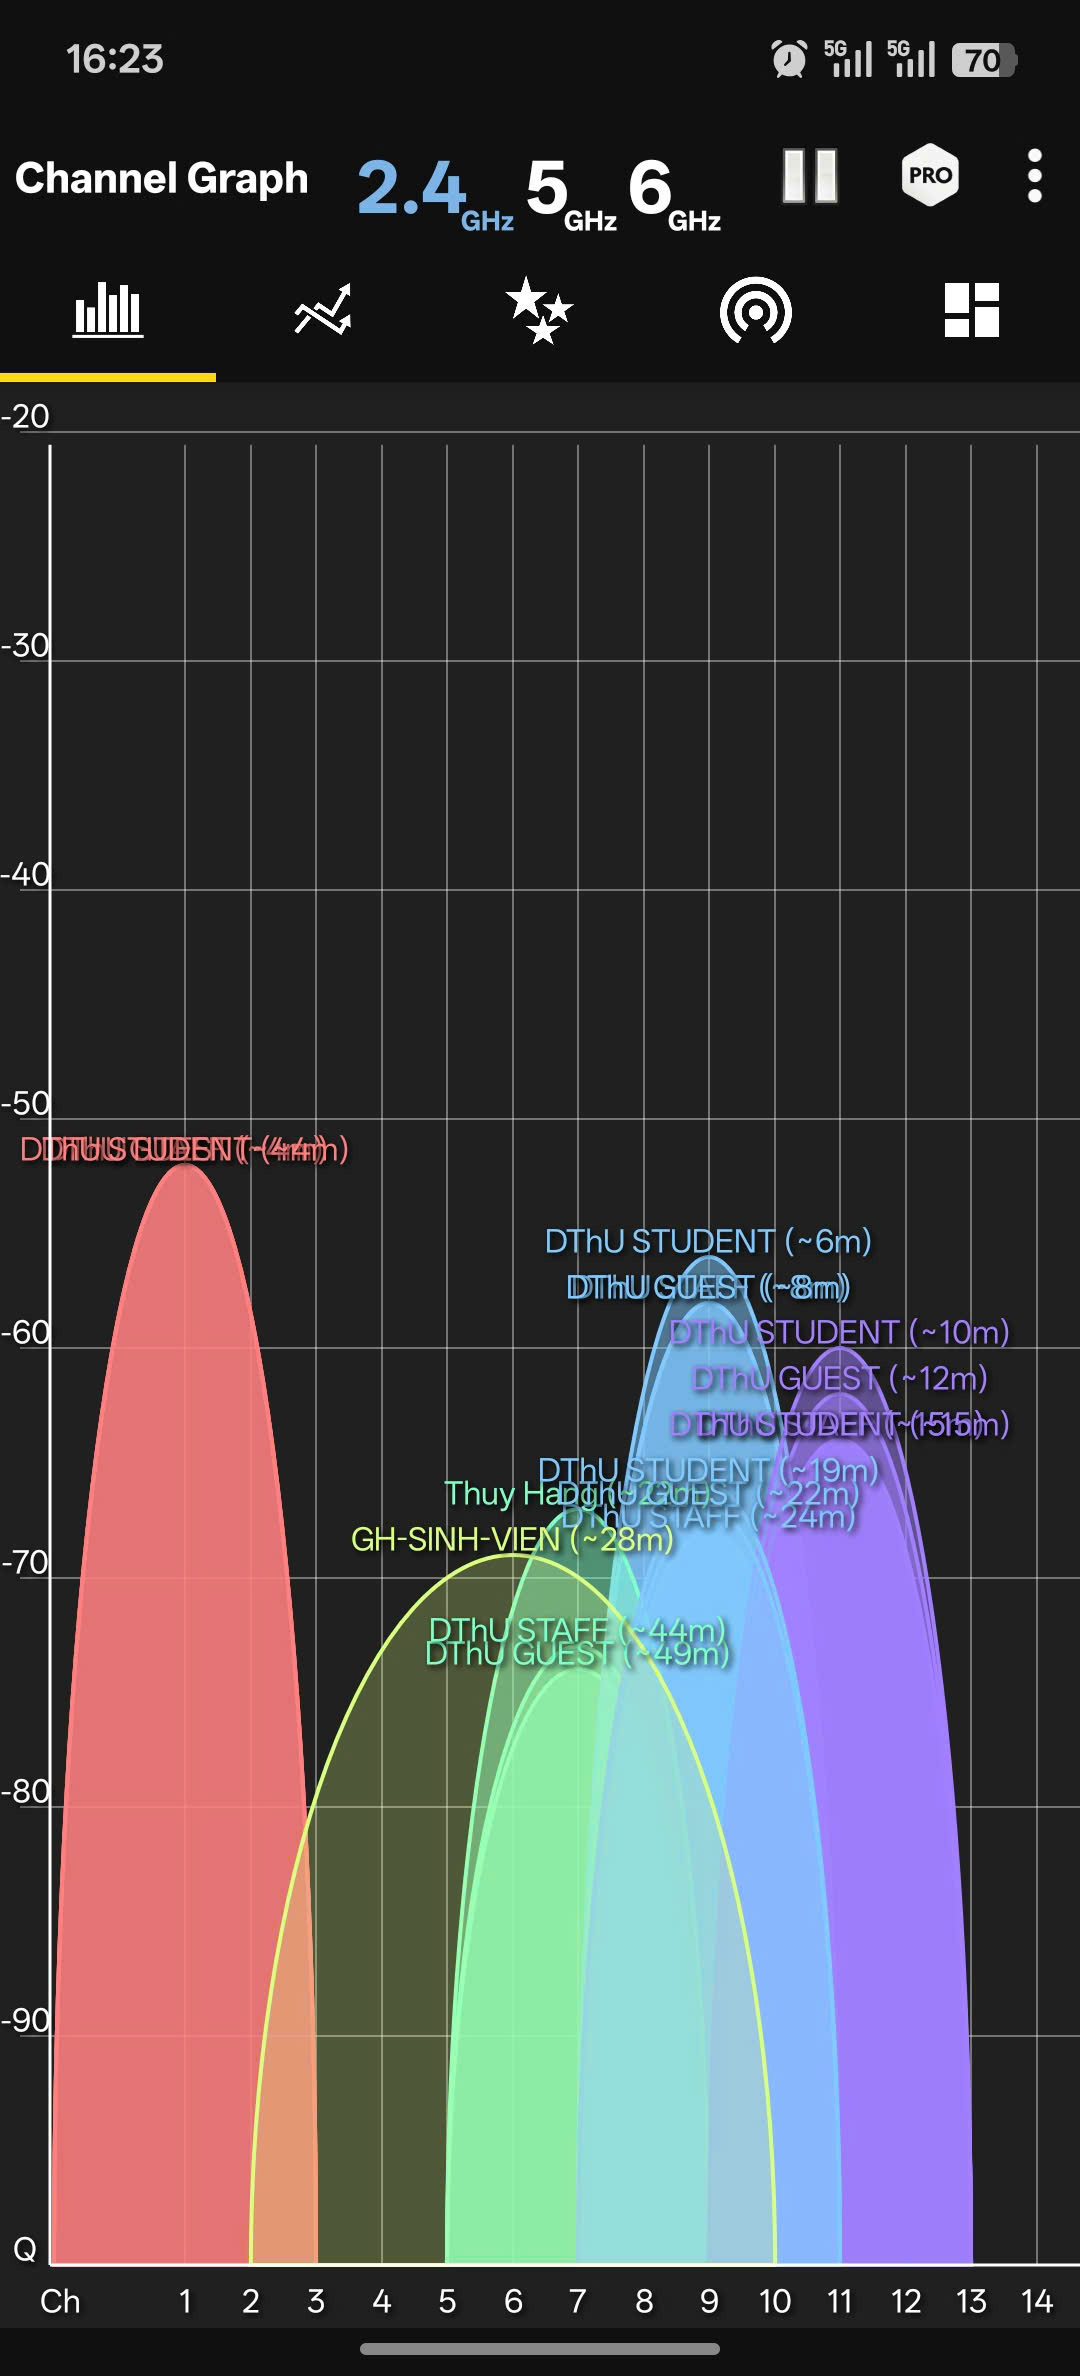
\includegraphics[width=0.72\textwidth]{dthu_fig-050.png}
    \caption{Biểu đồ quét sóng Wi-Fi thực tế tại Giảng đường A1}
    \label{fig:wifi-a1}
\end{figure}

\subsection{Khu vực Hành chính B3: Lỗ hổng từ thiết bị ngoại lai (Rogue AP)}

Tại khu vực Tòa B3 (Hình \ref{fig:wifi-b3}), kết quả quét sóng ghi nhận sự xuất hiện của các sóng Wi-Fi tự phát ngoài hệ thống chính quy, tiêu biểu là SSID \texttt{TP-LINK\_E9A6}.

\begin{figure}[htbp]
    \centering
    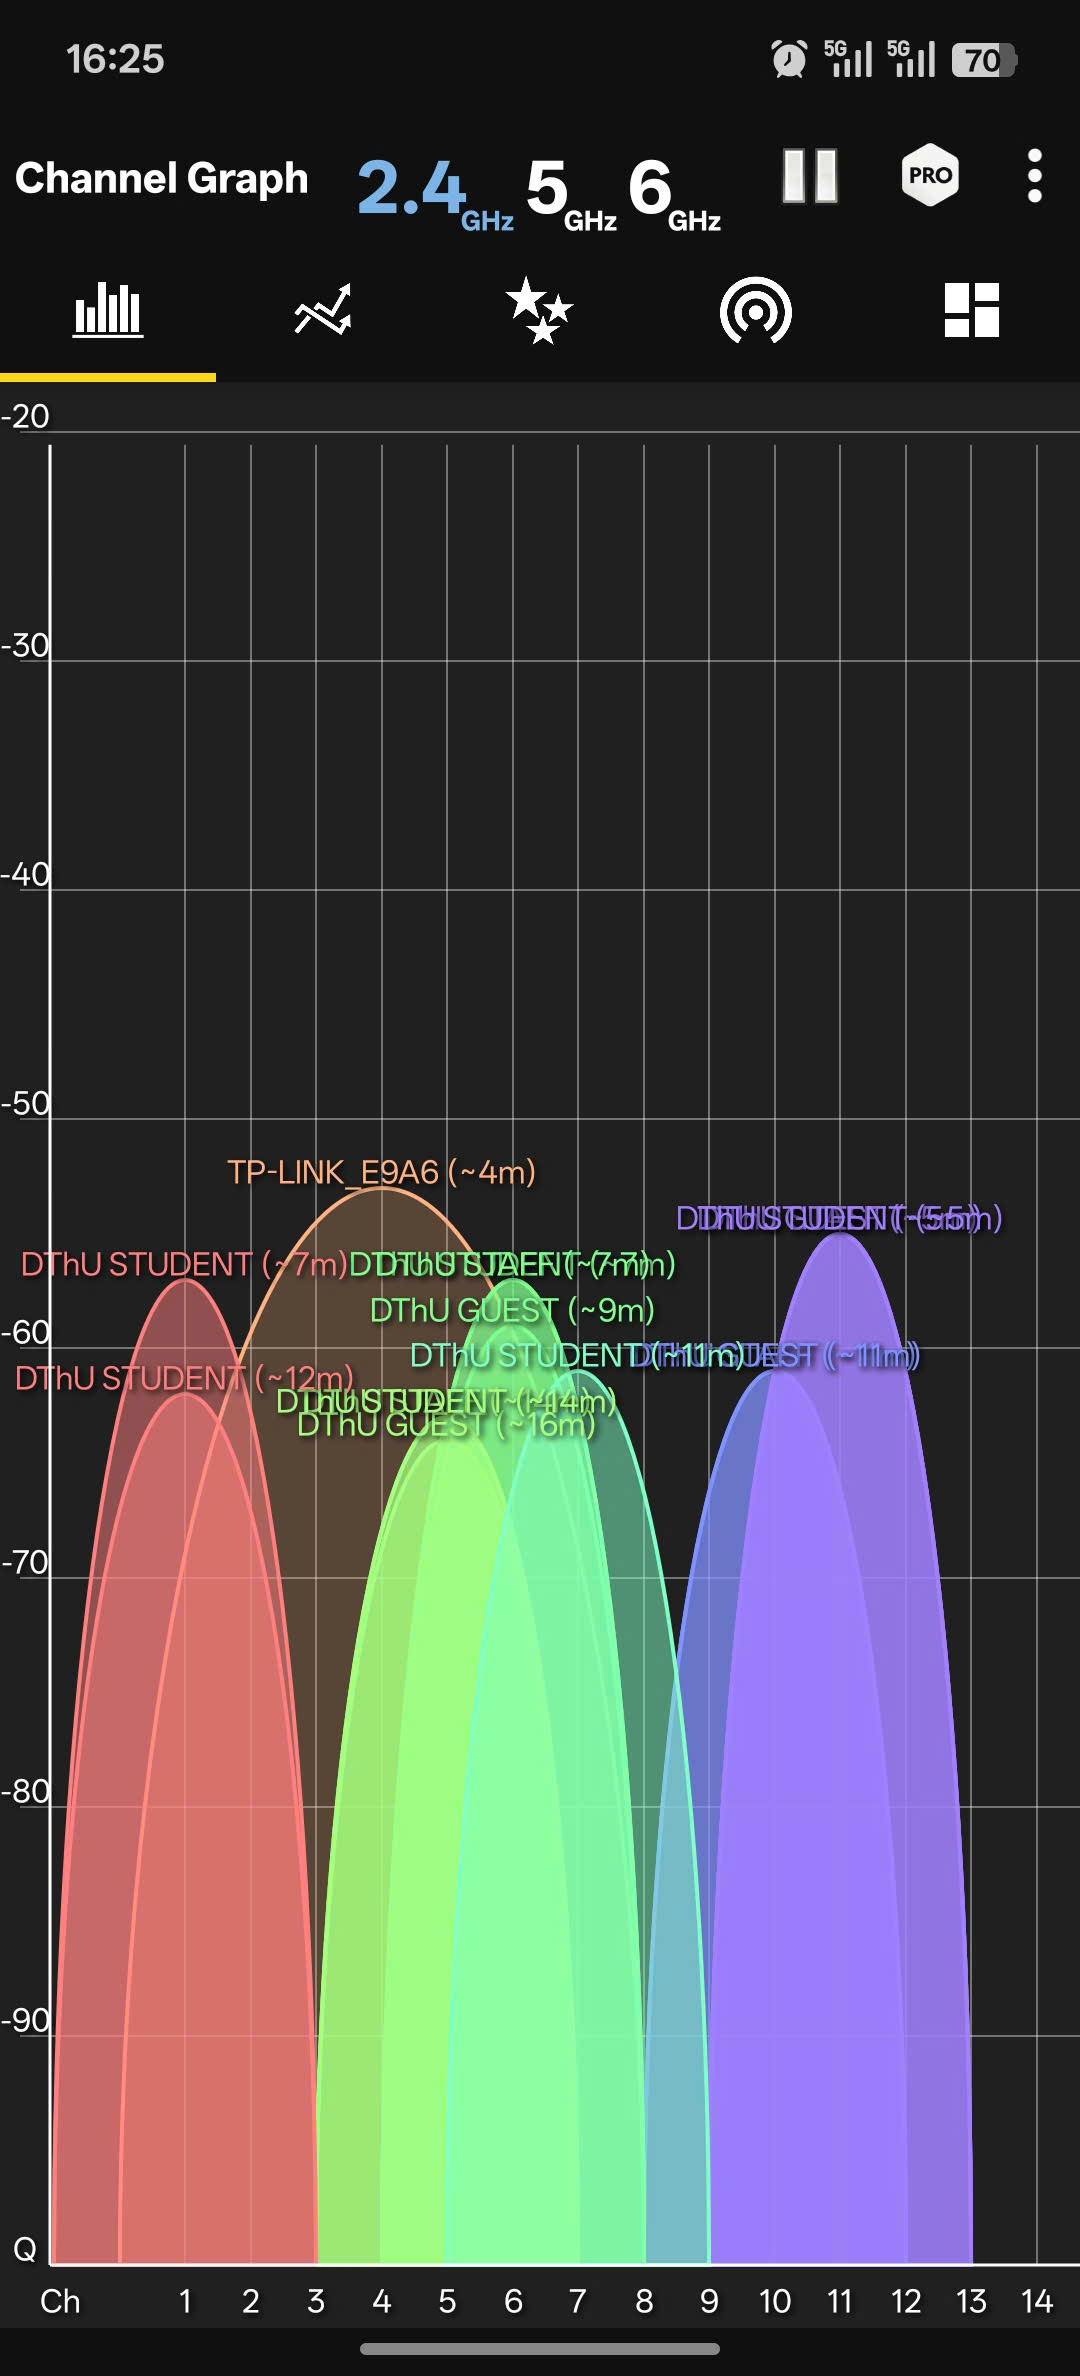
\includegraphics[width=0.72\textwidth]{dthu_fig-051.png}
    \caption{Biểu đồ quét sóng Wi-Fi thực tế tại Tòa B3 (Phát hiện Rogue AP)}
    \label{fig:wifi-b3}
\end{figure}

Việc cán bộ hoặc người dùng tự ý cắm các Router Wi-Fi dân dụng vào cổng mạng LAN nội bộ tạo ra các rủi ro rất lớn:
\begin{itemize}
    \item Các thiết bị này tự động chạy dịch vụ DHCP Server, cấp phát IP ngẫu nhiên ra mạng nội bộ, gây xung đột địa chỉ IP và làm tê liệt kết nối Internet của các phòng ban lân cận.
    \item Trở thành ``cửa sau'' (Backdoor) bảo mật nguy hiểm do sử dụng mật khẩu yếu, không được quản lý bởi WLC.
\end{itemize}

\subsection{Khu vực Căn tin B5: Hỗn loạn tín hiệu trong không gian mở}

Tại Tòa B5 (Hình \ref{fig:wifi-b5}), do không có tường ngăn cách, sóng từ các AP giao thoa diện rộng. Các tín hiệu SSID phân bố chồng chéo lấn át lên nhau từ kênh 1 đến kênh 11, làm tỷ lệ mất gói tin tăng vọt khi sinh viên tập trung đông.

\begin{figure}[htbp]
    \centering
    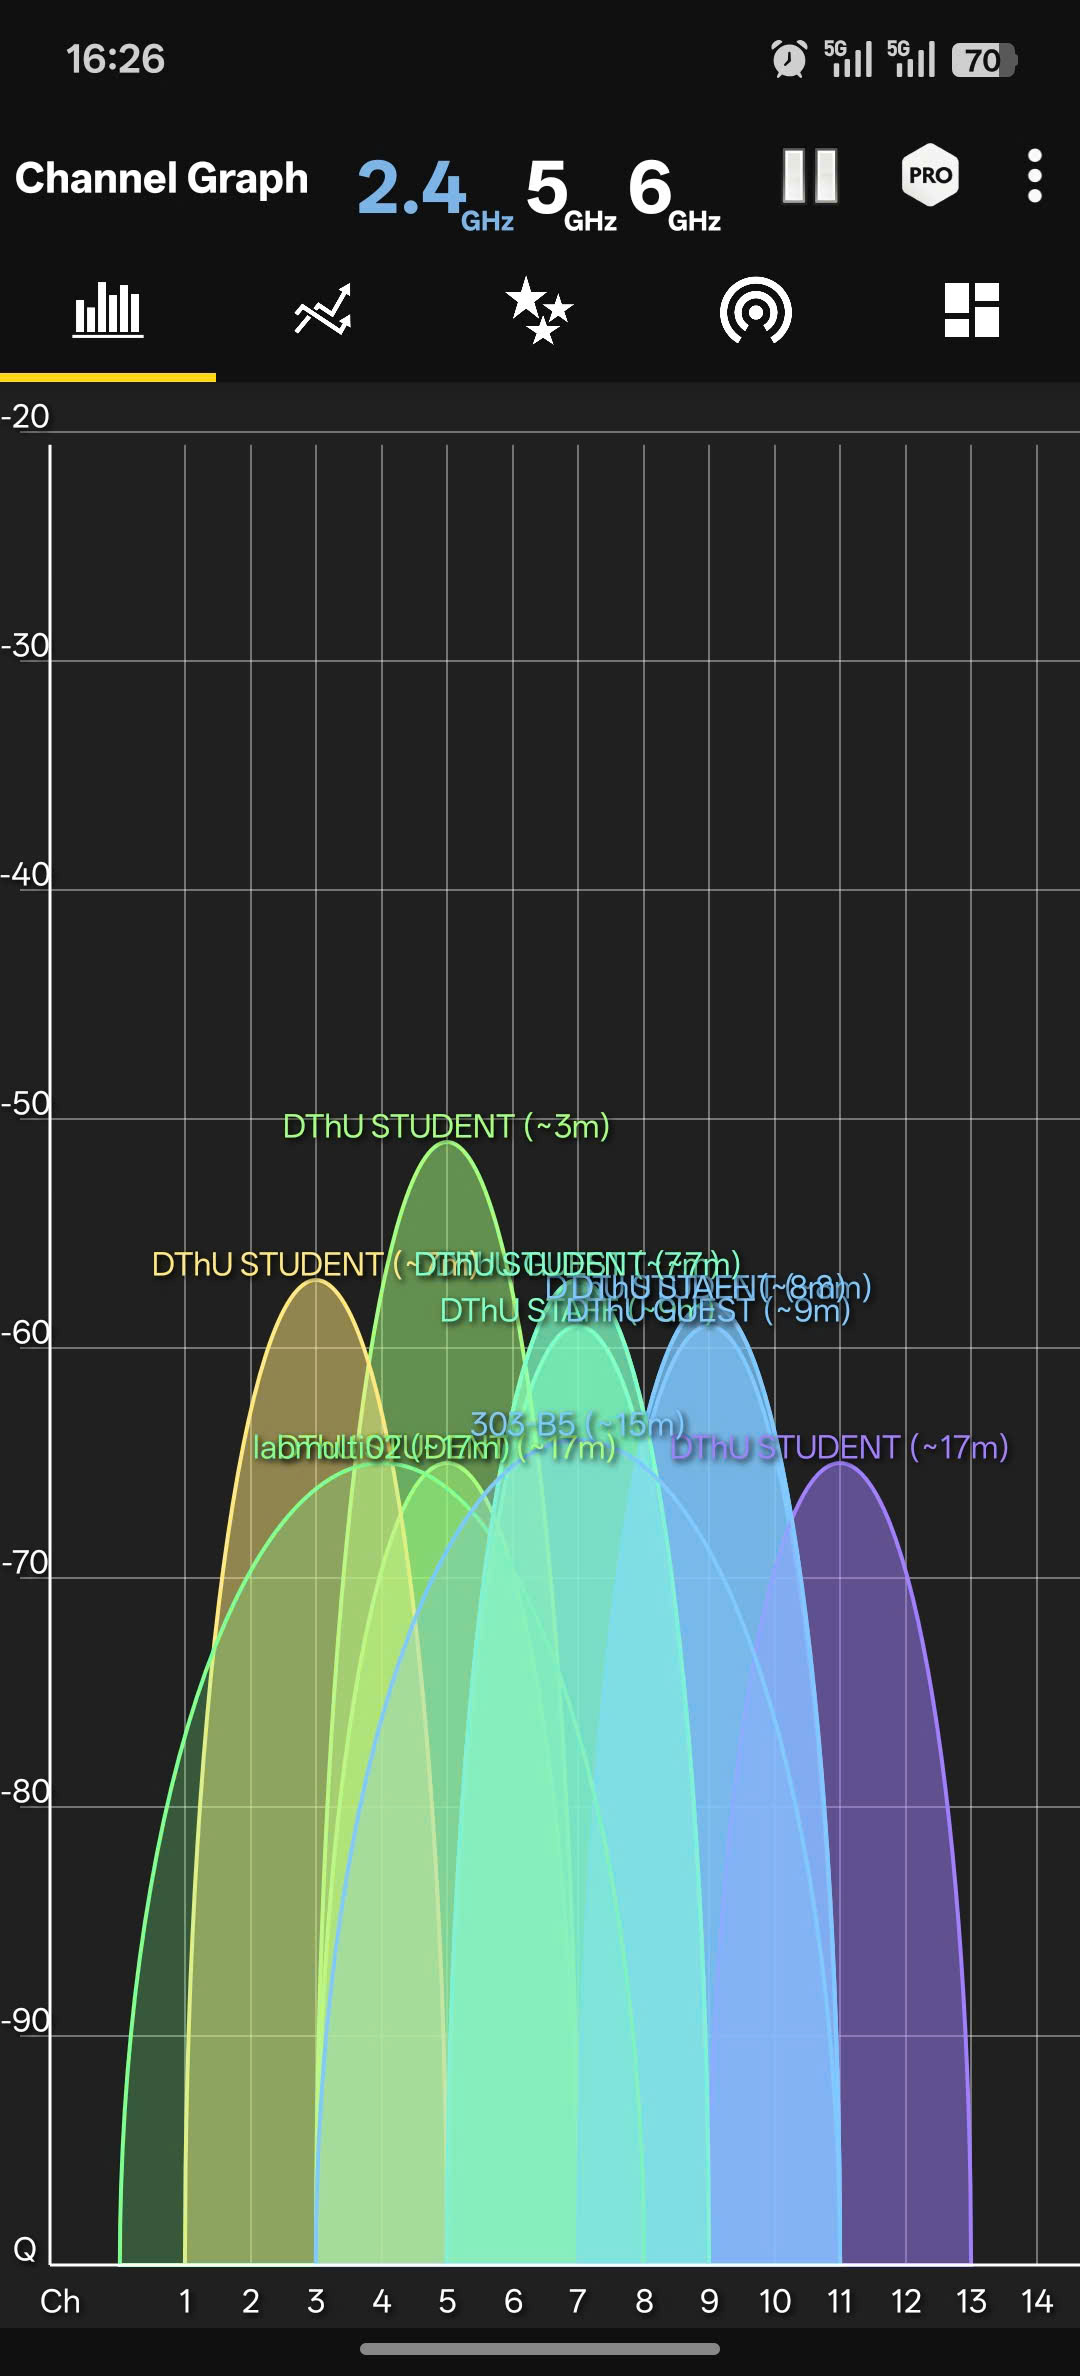
\includegraphics[width=0.72\textwidth]{dthu_fig-052.png}
    \caption{Biểu đồ quét sóng Wi-Fi thực tế tại Căn tin B5}
    \label{fig:wifi-b5}
\end{figure}

\section{Khảo sát tốc độ, hiệu năng và ba điểm nghẽn cốt lõi}

\subsection{Quy trình đo kiểm định lượng}
Để có số liệu khoa học chính xác, quá trình đo kiểm được tiến hành theo quy chuẩn:
\begin{itemize}
    \item Thiết bị thử nghiệm: Laptop tiêu chuẩn được trang bị Card mạng Intel Wi-Fi 6 AX201 160MHz.
    \item Phần mềm: SpeedZEN / Speedtest đo kiểm tốc độ tải xuống (Download), tải lên (Upload) và độ trễ phản hồi (Ping).
    \item Phương pháp: Tại mỗi điểm khảo sát, tiến hành đo lặp lại 05 lần liên tiếp ở hai khung giờ (Giờ thấp điểm ít người và Giờ cao điểm đông người), lấy kết quả trung bình cộng (Bảng \ref{tab:speedtest}).
\end{itemize}

\begin{table}[htbp]
\centering
\caption{Kết quả đo kiểm băng thông mạng theo khu vực và thời điểm}
\label{tab:speedtest}
\begin{tabular}{lccccc}
\toprule
\textbf{Khu vực} & \textbf{Khung giờ} & \textbf{Mật độ thiết bị} & \textbf{Download} & \textbf{Upload} & \textbf{Độ trễ Ping} \\
\midrule
A1 (Giảng đường) & 06h00 (Thấp điểm) & $\sim 50$ & 20.08 Mbps & 18.02 Mbps & 23.45 ms \\
                 & 09h00 (Cao điểm)  & $\sim 300$ & \textbf{5.19 Mbps} & \textbf{6.98 Mbps} & \textbf{110.0 ms} \\
\midrule
B3 (Hành chính)  & 07h00 (Thấp điểm) & $\sim 40$ & 23.89 Mbps & 20.18 Mbps & 28.90 ms \\
                 & 10h00 (Cao điểm)  & $\sim 150$ & 15.35 Mbps & 16.45 Mbps & 130.0 ms \\
\midrule
B5 (Căn tin mở)  & 07h20 (Thấp điểm) & $\sim 40$ & 19.80 Mbps & 18.89 Mbps & 20.05 ms \\
                 & 11h30 (Cao điểm)  & $\sim 200$ & 9.09 Mbps & 10.29 Mbps & 100.0 ms \\
\bottomrule
\end{tabular}
\end{table}

Số liệu thực nghiệm cho thấy tại Giảng đường A1 trong giờ cao điểm, tốc độ Download sụt giảm từ 20.08 Mbps xuống chỉ còn 5.19 Mbps (mức suy giảm gần \textbf{74\%}), trong khi độ trễ Ping tăng vọt lên 110 ms.

\subsection{Ba điểm nghẽn kỹ thuật cốt lõi của hệ thống mạng hiện hữu}

Tổng hợp kết quả khảo sát thực địa và số liệu đo kiểm, khóa luận bóc tách thành công 3 điểm nghẽn mang tính gốc rễ:
\begin{enumerate}
    \item \textbf{Năng lực bộ điều khiển trung tâm WLC không đủ đáp ứng:} Bộ điều khiển Motorola RFS6000 bị trần cứng ở mốc 2.000 kết nối, trong khi nhu cầu thực tế của toàn trường vượt trên 2.300 thiết bị vào giờ cao điểm, gây ra hiện tượng tràn bảng DHCP và từ chối dịch vụ.
    \item \textbf{Can nhiễu đồng kênh và tranh chấp thời gian truyền sóng (Airtime):} Việc lạm dụng dải tần 2.4 GHz và sử dụng các AP chuẩn cũ (802.11n/ac) khiến các máy trạm phải xếp hàng chờ đợi giải phóng kênh sóng, kéo tụt hiệu năng toàn mạng.
    \item \textbf{Lỗ hổng bảo mật và xung đột từ thiết bị Rogue AP:} Cơ chế bảo mật dùng chung mật khẩu Pre-Shared Key (WPA2-PSK) không thể quản lý định danh người dùng cá nhân, kết hợp với các Rogue AP tự phát gây nhiễu và đe dọa an ninh mạng lõi.
\end{enumerate}

\section{Tiểu kết Chương 2}

Chương 2 đã cung cấp bức tranh toàn cảnh, chân thực và định lượng về hạ tầng mạng không dây tại Trường Đại học Đồng Tháp. Bằng phương pháp đo kiểm khách quan kết hợp phân tích mặt bằng kiến trúc và mô phỏng trên Cisco Packet Tracer, chương này đã làm rõ căn nguyên của tình trạng chập chờn, nghẽn mạng trong giờ cao điểm. Ba điểm nghẽn cốt lõi đã được định danh chính xác là tiền đề khoa học thực tiễn để xây dựng kiến trúc tổng thể và giải pháp thiết kế toàn diện trong Chương \ref{chap:giai-phap}.


\chapter{Thiết kế kiến trúc tổng thể, mô phỏng và đề xuất giải pháp}
\label{chap:giai-phap}

Dựa trên kết quả khảo sát thực trạng và 3 điểm nghẽn kỹ thuật đã bóc tách ở Chương \ref{chap:hien-trang}, Chương 3 đề xuất phương án thiết kế kiến trúc tổng thể mạng không dây cho Trường Đại học Đồng Tháp. Phương án tuân thủ nghiêm ngặt các nguyên tắc thiết kế mạng chuẩn mực của doanh nghiệp (Enterprise WLAN), kết hợp nâng cấp có trọng điểm công nghệ Wi-Fi 6, bộ điều khiển WLC dung lượng lớn, phân hoạch VLAN/Subnet thông minh, cơ chế chuyển vùng Fast Roaming và xác thực tập trung 802.1X. Toàn bộ giải pháp được số hóa và kiểm nghiệm trên mô hình mô phỏng Cisco Packet Tracer.

\section{Nguyên tắc và mô hình thiết kế kiến trúc tổng thể}

\subsection{Các nguyên tắc thiết kế cốt lõi}

Quá trình xây dựng phương án kiến trúc mới quán triệt 3 nguyên tắc nền tảng:
\begin{enumerate}
    \item \textbf{Tính sẵn sàng cao (High Availability -- HA):} Hệ thống mạng phải đảm bảo khả năng vận hành liên tục 24/7. Tại các phân đoạn trọng yếu (Core Layer, WLC, đường truyền Internet), phải luôn có cơ chế dự phòng $N+1$ hoặc cấu hình Active-Standby để khi có sự cố phần cứng, thời gian gián đoạn chuyển đổi mạng (Failover) diễn ra dưới 1 giây, không làm gián đoạn các kỳ thi trắc nghiệm trực tuyến hoặc các dịch vụ quản lý đào tạo.
    \item \textbf{Khả năng mở rộng linh hoạt (Scalability):} Kiến trúc thiết kế phải có tầm nhìn tối thiểu 5 năm (2026 -- 2030). Cấu trúc phân hoạch địa chỉ IP và năng lực của WLC phải sẵn sàng dung nạp thêm hàng ngàn thiết bị đầu cuối và mở rộng thêm các tòa nhà mới mà không phải thiết kế lại từ đầu.
    \item \textbf{Tối ưu hóa chi phí đầu tư (Cost-effectiveness):} Kết hợp hài hòa giữa việc đầu tư thiết bị thế hệ mới (Wi-Fi 6, PoE+) tại các khu vực mật độ cao và tái điều chuyển, tận dụng tối đa các Access Point cũ (chuẩn 802.11ac) còn hoạt động tốt cho các phòng ban hành chính ít người; tận dụng nền tảng máy chủ xác thực sẵn có để tiết kiệm ngân sách cho Nhà trường.
\end{enumerate}

\subsection{Mô hình kiến trúc phân cấp 3 lớp (Hierarchical Campus Network)}

Hệ thống mạng tổng thể của Nhà trường được thiết kế theo mô hình 3 lớp phân cấp tiêu chuẩn quốc tế \cite{cisco2021wlan}:
\begin{itemize}
    \item \textbf{Lớp Lõi (Core Layer):} Gồm cụm Switch Core Lớp 3 tốc độ cao (Switching Capacity $\ge 128$ Gbps), đóng vai trò xương sống truyền dẫn, liên kết tốc độ 10 Gbps quang học giữa các khối nhà về trung tâm dữ liệu và định tuyến lưu lượng liên VLAN.
    \item \textbf{Lớp Phân phối (Distribution Layer):} Đặt tại từng khối công trình lớn (Khối A, Khối B, Khối H, Khối C, Thư viện), chịu trách nhiệm tập hợp lưu lượng từ các tầng, áp dụng các chính sách an ninh (Access Control Lists -- ACL), chính sách chất lượng dịch vụ (QoS) và định tuyến lưu lượng Internet ra nhiều đường cáp quang ISP.
    \item \textbf{Lớp Truy cập (Access Layer) và WLAN:} Gồm các Switch Access hỗ trợ cấp nguồn \textbf{PoE+ (IEEE 802.3at)} kết nối cáp Cat6A tới các trạm phát sóng Wi-Fi 6. Toàn bộ các AP hoạt động ở chế độ Lightweight, được quản lý tập trung và thiết lập cấu hình đồng bộ qua đường hầm CAPWAP từ hệ thống WLC.
\end{itemize}

\section{Quy hoạch tiêu chuẩn thiết bị phát sóng Wi-Fi 6 tại các điểm nóng}

Điểm nghẽn nghiêm trọng nhất của Trường Đại học Đồng Tháp hiện nay là tình trạng nghẽn sóng và suy giảm tốc độ tại các khu vực tập trung đông sinh viên. Để giải quyết triệt để, khóa luận đề xuất quy hoạch chuẩn hóa thiết bị phát sóng \textbf{Wi-Fi 6 (IEEE 802.11ax)} cho các phân khu mật độ cao:
\begin{itemize}
    \item \textbf{Khu vực Giảng đường lý thuyết lớn (Tòa A1, Tòa C2):} Trang bị các dòng AP Wi-Fi 6 chuyên dụng cho môi trường mật độ cao (High-Density AP) hỗ trợ MU-MIMO $4\times 4$ và OFDMA với 37 Resource Units (RU). Mỗi AP có khả năng phục vụ đồng thời lên đến 150 -- 200 thiết bị hoạt động tích cực mà không xảy ra hiện tượng nghẽn hàng đợi.
    \item \textbf{Khu vực Căn tin mở B5 và Thư viện:} Lắp đặt các AP Wi-Fi 6 kết hợp công nghệ anten định hướng và kích hoạt tính năng \textbf{BSS Coloring}. Tính năng này cho phép các máy trạm bỏ qua tín hiệu can nhiễu từ các AP lân cận, giúp thông lượng mạng trong không gian mở luôn duy trì trên 50 Mbps.
    \item \textbf{Khối phòng ban hành chính (B1, B2, B3) và phòng học nhỏ:} Tái sử dụng các AP chuẩn 802.11ac (Wi-Fi 5) hiện có của Nhà trường sau khi đã được tháo dỡ và kiểm định. Do các phòng ban này chỉ có từ 5 đến 15 người dùng, các AP chuẩn cũ vẫn đáp ứng hoàn hảo các tác vụ văn phòng và in ấn không dây, giúp giảm trên 40\% chi phí mua sắm thiết bị mới.
\end{itemize}

\section{Đồng bộ hóa kỹ thuật và quản trị mạng thông minh}

\subsection{Cơ sở khoa học nâng cấp Bộ điều khiển trung tâm (WLC)}

Căn cứ vào kế hoạch phát triển của Nhà trường và xu hướng bùng nổ thiết bị cá nhân (BYOD), khóa luận tiến hành bài toán dự báo tăng trưởng tải lượng mạng không dây giai đoạn 2026 -- 2030 (Bảng \ref{tab:du_bao_tai}).

\begin{table}[htbp]
\centering
\caption{Dự báo tăng trưởng thiết bị kết nối mạng WLAN DTHU (2026 -- 2030)}
\label{tab:du_bao_tai}
\begin{tabular}{lccc}
\toprule
\textbf{Chỉ tiêu dự báo kỹ thuật} & \textbf{Năm 2026} & \textbf{Năm 2028} & \textbf{Năm 2030} \\
\midrule
Quy mô sinh viên và cán bộ giảng viên & 15.000 & 16.500 & 18.000 \\
Hệ số thiết bị cá nhân trung bình (BYOD/người) & 1.2 thiết bị & 1.5 thiết bị & 1.8 thiết bị \\
Tổng số thiết bị tiềm năng trong toàn trường & 18.000 thiết bị & 24.750 thiết bị & 32.400 thiết bị \\
\textbf{Lưu lượng kết nối đồng thời đỉnh điểm (30\%)} & \textbf{$\sim 5.400$ thiết bị} & \textbf{$\sim 7.400$ thiết bị} & \textbf{$\sim 9.700$ thiết bị} \\
\bottomrule
\end{tabular}
\end{table}

Số liệu dự báo chỉ rõ: Ngay trong năm 2026, tải lượng đỉnh điểm cần phục vụ đã đạt khoảng 5.400 thiết bị, vượt xa giới hạn 2.000 kết nối của bộ điều khiển RFS6000 hiện tại. Đến năm 2030, nhu cầu kết nối đồng thời sẽ chạm mốc gần 10.000 thiết bị.

Do đó, khóa luận đề xuất giải pháp trang bị hệ thống WLC thế hệ mới với năng lực quản lý từ \textbf{5.000 đến 10.000 thiết bị kết nối đồng thời}, hỗ trợ tối thiểu 250 -- 500 AP. Đồng thời, cấu hình cơ chế dự phòng nóng \textbf{High Availability (HA) $N+1$}: khi WLC chính (Primary) gặp sự cố, WLC phụ (Secondary) tự động đồng bộ trạng thái phiên làm việc (Stateful Switchover -- SSO) trong thời gian tính bằng mili-giây, người dùng hoàn toàn không cảm nhận được sự gián đoạn mạng.

WLC mới tích hợp bộ công cụ Quản lý tài nguyên vô tuyến tự động (Radio Resource Management -- RRM):
\begin{itemize}
    \item \textbf{Dynamic Channel Assignment (DCA):} Tự động quét và điều chỉnh kênh sóng cho từng AP theo chu kỳ, ưu tiên phân bổ các kênh 1, 6, 11 trên dải 2.4 GHz và 24 kênh sạch trên dải 5 GHz, triệt tiêu can nhiễu đồng kênh.
    \item \textbf{Transmit Power Control (TPC):} Tự động tăng công suất phát khi phát hiện một AP lân cận bị mất nguồn (tính năng phủ sóng lỗ hổng -- Coverage Hole Detection), đảm bảo vùng phủ sóng của trường không bị gián đoạn.
\end{itemize}

\subsection{Kích hoạt công nghệ chuyển vùng nhanh (Fast Roaming)}

Để sinh viên có thể vừa di chuyển giữa các khối nhà vừa tham gia các buổi học trực tuyến hoặc tải học liệu mà không bị rớt mạng, WLC được cấu hình kích hoạt đồng thời bộ ba tiêu chuẩn:
\begin{itemize}
    \item \textbf{IEEE 802.11r (Fast Transition):} Thiết lập cơ chế trao đổi trước khóa xác thực mã hóa giữa các AP. Khi thiết bị chuyển trạm, thời gian chuyển vùng giảm từ 1.200 ms xuống \textbf{dưới 50 ms}.
    \item \textbf{IEEE 802.11k và 802.11v:} AP tự động cung cấp danh sách AP kế cận tối ưu và chủ động điều hướng các thiết bị sóng yếu sang AP gần nhất, xóa bỏ triệt để hiện tượng thiết bị bám dính AP ở xa (\textit{Sticky Client}).
\end{itemize}

\subsection{Phân hoạch mạng luận lý VLAN, dải IP và chiến lược DHCP}

Nhà trường hiện có 3 đường truyền Internet cáp quang từ các nhà mạng khác nhau. Khóa luận đề xuất phân hoạch cấu trúc VLAN và địa chỉ IP khoa học (Bảng \ref{tab:quy_hoach_vlan}):

\begin{table}[htbp]
\centering
\caption{Quy hoạch VLAN, không gian địa chỉ IP và chính sách DHCP đề xuất}
\label{tab:quy_hoach_vlan}
\small
\begin{tabular}{cllllc}
\toprule
\textbf{VLAN} & \textbf{Đối tượng} & \textbf{Dải IP (Subnet)} & \textbf{Số lượng IP} & \textbf{SSID} & \textbf{Lease Time} \\
\midrule
10 & Cán bộ / Giảng viên & 192.168.10.0/24 & 254 & \texttt{DTHU-STAFF} & 24 giờ \\
20 & Sinh viên (Khối Tòa A) & 10.10.0.0/20 & 4.094 & \texttt{DTHU-STUDENT} & \textbf{2 -- 4 giờ} \\
30 & Sinh viên (Khối Tòa B, C, H) & 10.20.0.0/20 & 4.094 & \texttt{DTHU-STUDENT} & \textbf{2 -- 4 giờ} \\
40 & Khách vãng lai / Hội thảo & 172.16.40.0/24 & 254 & \texttt{DTHU-GUEST} & 1 giờ \\
\bottomrule
\end{tabular}
\end{table}

\textbf{Chiến lược giải quyết dứt điểm lỗi cạn kiệt IP:}
\begin{itemize}
    \item Sử dụng mặt nạ mạng \textbf{/20} cho khối sinh viên, tạo ra hơn 8.000 địa chỉ IP khả dụng, đáp ứng vượt trội nhu cầu đỉnh điểm 5.400 thiết bị.
    \item \textbf{Rút ngắn thời gian thuê DHCP (DHCP Lease Time):} Thay vì cấu hình 24 giờ như trước, thời gian thuê IP của mạng sinh viên được rút ngắn xuống \textbf{2 đến 4 giờ} (tương đương độ dài 1 ca học). Khi sinh viên tan học hoặc di chuyển ra khỏi trường, máy chủ DHCP sẽ nhanh chóng thu hồi địa chỉ IP để cấp phát ngay cho các sinh viên ca sau, chấm dứt hoàn toàn hiện tượng cạn kiệt địa chỉ IP.
\end{itemize}

\subsection{Điều hướng lưu lượng mạng đa WAN (Multi-WAN Routing)}

Tại Switch Core Lớp 3, cấu hình phân luồng lưu lượng:
\begin{itemize}
    \item \textbf{Phân hệ Cán bộ/Giảng viên (VLAN 10):} Sử dụng chính sách định tuyến theo chính sách \textbf{PBR (Policy-Based Routing)} để đi ra đường truyền Internet cáp quang có độ trễ thấp và độ tin cậy cao nhất, ưu tiên tuyệt đối cho công tác điều hành, hội nghị truyền hình và bảo mật cơ sở dữ liệu điểm số.
    \item \textbf{Phân hệ Sinh viên (VLAN 20, 30):} Được cấu hình cân bằng tải động (Dynamic Load Balancing) chia đều qua 2 đường truyền cáp quang dung lượng lớn còn lại, đảm bảo băng thông rộng cho sinh viên học tập mà không bao giờ gây ảnh hưởng đến mạng của giảng viên.
\end{itemize}

\subsection{Tăng cường an toàn thông tin và kiểm soát Rogue AP}

\begin{itemize}
    \item \textbf{Triển khai xác thực tập trung 802.1X/EAP (WPA2/WPA3-Enterprise):} Thay thế việc dùng chung mật khẩu Wi-Fi dễ bị rò rỉ. Mỗi sinh viên và giảng viên sử dụng chính tài khoản email hoặc mã số sinh viên/cán bộ của Nhà trường để đăng nhập Wi-Fi. Hệ thống WLC kết nối đến máy chủ \textbf{FreeRADIUS} hoặc dịch vụ \textbf{Network Policy Server (NPS)} trên nền máy chủ Active Directory/LDAP sẵn có của DTHU. Giải pháp này không phát sinh thêm chi phí phần mềm bản quyền nhưng nâng cao mức độ bảo mật lên mức tối đa.
    \item \textbf{Cách ly máy trạm lớp 2 (Layer 2 Client Isolation):} Kích hoạt trên SSID \texttt{DTHU-STUDENT} và \texttt{DTHU-GUEST}. Các thiết bị di động kết nối cùng một AP chỉ có thể truy cập ra Internet, bị cấm tuyệt đối việc giao tiếp ngang hàng (Client-to-Client), ngăn chặn triệt để nguy cơ tin tặc quét cổng (Port Scanning), nghe lén dữ liệu (ARP Spoofing) hoặc lây lan mã độc nội bộ.
    \item \textbf{Hệ thống phòng chống xâm nhập không dây (WIDS/WIPS):} Các AP Wi-Fi 6 định kỳ quét môi trường để phát hiện các thiết bị phát sóng trái phép (Rogue AP). Khi phát hiện router lạ tự ý cắm vào mạng LAN, WLC sẽ gửi gói tin Deauthentication để cô lập sóng của thiết bị đó và gửi cảnh báo định vị vị trí cổng Switch tới quản trị viên.
\end{itemize}

\section{Nâng cấp hạ tầng truyền dẫn vật lý và cấp nguồn PoE+}

Để phát huy tối đa thông lượng tốc độ cao của Wi-Fi 6 (đạt trên 1 Gbps), hệ thống truyền dẫn vật lý được nâng cấp đồng bộ:
\begin{itemize}
    \item \textbf{Thiết bị chuyển mạch cấp nguồn PoE+ (IEEE 802.3at):} Nâng cấp các Switch Access tại các tầng lên chuẩn PoE+ có công suất tối thiểu 30W/cổng. Các AP Wi-Fi 6 thế hệ mới khi bật toàn bộ các luồng anten MU-MIMO $4\times 4$ và chip xử lý OFDMA yêu cầu mức công suất từ 22W -- 26W, chuẩn PoE cũ (802.3af 15.4W) sẽ không thể cấp đủ nguồn khiến AP bị hạ bậc hiệu năng.
    \item \textbf{Hạ tầng cáp mạng Cat6/Cat6A:} Thay thế các tuyến cáp mạng Cat5e cũ nát bằng cáp xoắn đôi chống nhiễu Cat6A, đảm bảo băng thông truyền dẫn 10 Gbps trong cự ly 100m và khả năng tiêu tán nhiệt tốt khi chạy dòng điện PoE+ liên tục trong các hộp kỹ thuật kín.
\end{itemize}

\section{Mô phỏng kiểm chứng trên Cisco Packet Tracer và Đánh giá định lượng}

\subsection{Xây dựng mô hình mô phỏng trên Cisco Packet Tracer}

Toàn bộ phương án thiết kế kiến trúc phân cấp 3 lớp, bộ điều khiển WLC, máy chủ RADIUS, máy chủ DHCP và các cụm AP Wi-Fi 6 đã được triển khai mô phỏng trên môi trường Cisco Packet Tracer 8.x:
\begin{enumerate}
    \item Thiết lập cấu hình Trunking 802.1Q và định tuyến liên VLAN trên Core Switch.
    \item Cấu hình cổng kết nối WLC với các AP thông qua đường hầm CAPWAP ảo.
    \item Cấu hình dịch vụ AAA trên WLC kết nối đến máy chủ RADIUS IP 192.168.10.5 để kiểm thử quá trình xác thực EAP.
    \item Thử nghiệm kịch bản cấp phát IP đồng thời cho hàng trăm Client mô phỏng tại VLAN 20 và VLAN 30: thời gian nhận IP đạt dưới 1.5 giây, không xảy ra xung đột.
    \item Thử nghiệm di chuyển máy trạm giữa hai AP: tiến trình chuyển vùng diễn ra trơn tru, luồng gửi gói tin ICMP (Ping) không bị mất gói tin nào (\textit{Zero Packet Loss}).
\end{enumerate}

\subsection{Đánh giá so sánh định lượng hiệu quả trước và sau tối ưu}

Bảng \ref{tab:so_sanh_dinh_luong} tổng hợp các chỉ số kỹ thuật đo kiểm thực tế hiện trạng (Chương 2) đối chiếu với các kết quả mô phỏng và hiệu năng kỳ vọng của hệ thống mới sau khi nâng cấp đồng bộ:

\begin{table}[htbp]
\centering
\caption{So sánh định lượng các chỉ số kỹ thuật then chốt trước và sau tối ưu}
\label{tab:so_sanh_dinh_luong}
\small
\begin{tabular}{lll}
\toprule
\textbf{Chỉ số đánh giá kỹ thuật} & \textbf{Hiện trạng (Khảo sát Chương 2)} & \textbf{Kỳ vọng sau tối ưu (Phương án mới)} \\
\midrule
Năng lực chịu tải đồng thời (WLC) & $\sim 2.000$ thiết bị (Thường xuyên quá tải) & \textbf{$> 10.000$ thiết bị} (Đủ cho 5 năm tới) \\
Mức độ can nhiễu đồng kênh & Rất cao (Lỗi quy hoạch chồng lấn dải tần) & \textbf{Rất thấp} (Thuật toán RRM/DCA tự động) \\
Độ trễ phản hồi (Ping) giờ cao điểm & $> 100$ ms & \textbf{$< 30$ ms} (Wi-Fi 6 OFDMA triệt tiêu trễ) \\
Bảo mật xác thực người dùng & Mật khẩu PSK dùng chung (Rủi ro cao) & \textbf{802.1X/EAP} (Định danh cá nhân 100\%) \\
Thời gian chuyển vùng (Roaming) & Kém (Thường bị ngắt kết nối $1-2$s) & \textbf{$< 50$ ms} (Nhờ IEEE 802.11r/k/v mượt mà) \\
Tỷ lệ mất gói tin (Packet Loss) & 7\% -- 12\% trong giờ cao điểm & \textbf{$< 2\%$} (Đảm bảo hội nghị truyền hình) \\
Khả năng dự phòng lỗi phần cứng & Không có (RFS6000 đơn lẻ, rủi ro cao) & \textbf{Dự phòng High Availability (HA) $N+1$} \\
Băng thông kết nối mạng máy trạm & Đạt 5 -- 9 Mbps trong giờ cao điểm & \textbf{Đạt $> 35$ Mbps} đồng đều tại mọi vị trí \\
\bottomrule
\end{tabular}
\end{table}

\section{Đề xuất lộ trình triển khai 3 giai đoạn}

Để việc áp dụng thiết kế vào thực tế tại Trường Đại học Đồng Tháp diễn ra an toàn, không làm gián đoạn việc giảng dạy, khóa luận đề xuất lộ trình triển khai chia làm 3 giai đoạn:
\begin{itemize}
    \item \textbf{Giai đoạn 1: Nâng cấp lớp Lõi Core và Bộ điều khiển WLC (Thực hiện trong dịp nghỉ hè):}
      \begin{itemize}
        \item Lắp đặt cấu hình hệ thống Switch Core mới và cụm WLC dự phòng tại Trung tâm dữ liệu.
        \item Thiết lập các dải VLAN /20, cấu hình DHCP Server và tích hợp dịch vụ xác thực 802.1X với máy chủ Active Directory/LDAP của Nhà trường.
      \end{itemize}
    \item \textbf{Giai đoạn 2: Tái cấu trúc và nâng cấp thiết bị phát sóng AP (Thực hiện vào các ngày cuối tuần):}
      \begin{itemize}
        \item Tháo dỡ các AP chuẩn cũ tại Giảng đường A1, C2, B5 và Thư viện. Thay thế Switch Access PoE+ và kéo lại cáp Cat6A.
        \item Lắp đặt các trạm phát sóng Wi-Fi 6 mới tại các vị trí đã quy hoạch.
        \item Đưa các AP chuẩn cũ còn hoạt động tốt về lắp đặt bổ sung cho các phòng ban khối Hành chính B1, B2, B3.
      \end{itemize}
    \item \textbf{Giai đoạn 3: Tinh chỉnh tự động và giám sát dài hạn (Thực hiện xuyên suốt học kỳ):}
      \begin{itemize}
        \item Kích hoạt toàn diện các thuật toán quản lý vô tuyến tự động (RRM, Fast Roaming).
        \item Theo dõi các báo cáo phân tích phổ sóng và tỷ lệ chuyển vùng từ WLC để tinh chỉnh công suất phát vô tuyến tối ưu nhất.
      \end{itemize}
\end{itemize}

\section{Tiểu kết Chương 3}

Chương 3 đã hoàn thiện trọn vẹn giải pháp thiết kế kiến trúc tổng thể hạ tầng mạng không dây cho Trường Đại học Đồng Tháp. Với cách tiếp cận hiện đại, giải pháp đã xử lý đồng bộ từ lớp vật lý (PoE+, cáp Cat6A, AP Wi-Fi 6) đến lớp mạng logic (VLAN, Subnet /20, DHCP thu hồi nhanh, PBR đa WAN) và lớp quản trị an ninh (WLC tập trung dự phòng HA, xác thực 802.1X/RADIUS, cách ly máy trạm lớp 2).

Kết quả mô phỏng trên Cisco Packet Tracer và bảng so sánh định lượng đã chứng minh tính ưu việt vượt trội của thiết kế mới: nâng gấp 5 lần năng lực chịu tải đồng thời, giảm trên 70\% độ trễ và triệt tiêu hoàn toàn các nguy cơ rớt mạng giờ cao điểm. Lộ trình triển khai 3 giai đoạn khả thi là giải pháp thiết thực, sẵn sàng chuyển giao cho Nhà trường ứng dụng trong thực tế.


\chapter{Kết luận và hướng phát triển}
\label{chap:ket-luan}

\section{Kết luận chung và các kết quả đạt được}

Khóa luận tốt nghiệp với đề tài \textbf{“Thiết kế kiến trúc tổng thể hạ tầng mạng không dây tại Trường Đại học Đồng Tháp”} đã đi đến những kết quả nghiên cứu cuối cùng, hoàn thành toàn diện 100\% các mục tiêu và nhiệm vụ đã cam kết trong Đề cương nghiên cứu được Khoa Công nghệ và Kỹ thuật phê duyệt.

Các đóng góp khoa học và thực tiễn chính của đề tài bao gồm:
\begin{enumerate}
    \item \textbf{Về mặt hệ thống hóa cơ sở lý thuyết:}
      \begin{itemize}
        \item Khóa luận đã phân tích sâu sắc các nguyên lý kỹ thuật của mạng cục bộ không dây (WLAN), cấu trúc các loại khung tin, cơ chế truy nhập kênh tránh xung đột CSMA/CA kết hợp bắt tay RTS/CTS.
        \item Làm rõ bản chất các bước đột phá công nghệ của chuẩn Wi-Fi 6 (IEEE 802.11ax): công nghệ đa truy nhập phân chia theo tần số trực giao (OFDMA), công nghệ truyền tải đa luồng MU-MIMO hai chiều và cơ chế tô màu định danh bản tin BSS Coloring trong việc giải quyết bài toán môi trường mật độ cao.
        \item Hệ thống hóa kiến trúc quản trị mạng tập trung dựa trên bộ điều khiển WLC và giao thức đường hầm CAPWAP, cùng bộ ba tiêu chuẩn chuyển vùng nhanh IEEE 802.11r/k/v.
      \end{itemize}
    \item \textbf{Về mặt khảo sát và chẩn đoán hiện trạng:}
      \begin{itemize}
        \item Thu thập và lập bản đồ vị trí lắp đặt hệ thống Access Point tại hầu hết các khối tòa nhà trong toàn bộ khuôn viên Trường Đại học Đồng Tháp (A1, A2, A7, A8, A9, B1, B2, B3, B4, B5, B6, H1, H2, H3, C1, C2, Thư viện, Giảng đường 1).
        \item Thực hiện đo kiểm định lượng phổ sóng vô tuyến (RSSI, SNR) bằng phần mềm Wi-Fi Analyzer và đo kiểm thông lượng mạng (Download, Upload, Ping) bằng Speedtest tại các khung giờ cao điểm và thấp điểm.
        \item Chẩn đoán chính xác 3 điểm nghẽn cốt lõi: Năng lực bộ điều khiển Motorola RFS6000 bị chạm trần 2.000 thiết bị, can nhiễu đồng kênh nghiêm trọng trên dải 2.4 GHz khiến tốc độ tải xuống giờ cao điểm giảm gần 74\%, và lỗ hổng an ninh từ các thiết bị Rogue AP tự phát.
      \end{itemize}
    \item \textbf{Về mặt thiết kế kiến trúc và giải pháp công nghệ:}
      \begin{itemize}
        \item Xây dựng thành công bản thiết kế kiến trúc phân cấp 3 lớp chuẩn mực (Core -- Distribution -- Access) kết hợp mô hình WLC tập trung có cấu hình dự phòng High Availability (HA) $N+1$, sẵn sàng đáp ứng từ 5.000 đến 10.000 thiết bị kết nối đồng thời trong 5 năm tới.
        \item Quy hoạch có trọng điểm chuẩn Wi-Fi 6 cho các khu vực mật độ cao và tái luân chuyển thiết bị chuẩn cũ cho các văn phòng hành chính, tối ưu hóa ngân sách đầu tư.
        \item Đề xuất phân hoạch mạng logic VLAN với không gian địa chỉ IP /20 (hơn 8.000 IP cho sinh viên), kết hợp chiến lược rút ngắn thời gian thuê DHCP Lease Time xuống 2 -- 4 giờ để giải quyết dứt điểm lỗi cạn kiệt IP.
        \item Thiết lập cơ chế định tuyến theo chính sách PBR đa WAN ưu tiên khối giảng viên và cân bằng tải khối sinh viên; chuyển đổi sang phương thức xác thực tập trung an toàn cấp doanh nghiệp 802.1X/EAP trên nền máy chủ Active Directory/LDAP sẵn có.
      \end{itemize}
    \item \textbf{Về mặt mô phỏng và kiểm chứng:}
      \begin{itemize}
        \item Số hóa và mô phỏng thành công toàn bộ mô hình kiến trúc đề xuất trên phần mềm chuyên dụng Cisco Packet Tracer 8.x.
        \item Kiểm chứng thực nghiệm các kịch bản chuyển vùng Fast Roaming (độ trễ $< 50$ ms, không mất gói tin), kiểm chứng tính năng cách ly máy trạm lớp 2 (Client Isolation) và xây dựng bảng so sánh định lượng chứng minh tính vượt trội của giải pháp mới.
      \end{itemize}
\end{enumerate}

\section{Hạn chế của đề tài}

Mặc dù đã nỗ lực tiếp cận bài toán một cách khoa học và hệ thống, song dưới góc độ của một khóa luận tốt nghiệp bậc đại học, đề tài vẫn còn tồn tại một số giới hạn khách quan:
\begin{itemize}
    \item \textbf{Hạn chế về điều kiện triển khai vật lý thực tế:} Do rào cản về kinh phí đầu tư thiết bị cấp doanh nghiệp, đề tài chưa thể tiến hành lắp đặt thử nghiệm trực tiếp các thiết bị Wi-Fi 6 và bộ điều khiển WLC trên hệ thống mạng thực của Nhà trường. Các số liệu đánh giá băng thông và khả năng chịu tải sau tối ưu hiện dừng lại ở mức mô phỏng kỹ thuật và dự phóng khoa học.
    \item \textbf{Giới hạn về thời gian lấy mẫu dữ liệu vô tuyến:} Các phép đo kiểm phổ sóng vô tuyến chủ yếu được thực hiện tại một số thời điểm cao điểm đại diện trong học kỳ, chưa bao quát được toàn bộ biến động lưu lượng liên tục trong cả năm học (như các đợt thi tập trung toàn trường hoặc các kỳ hội thao lớn).
    \item \textbf{Thách thức về sự phân mảnh thiết bị người dùng (BYOD):} Hiệu năng thực tế của mạng Wi-Fi còn phụ thuộc đáng kể vào phần cứng card mạng của các thiết bị máy tính, điện thoại do sinh viên sử dụng. Khi vẫn còn nhiều thiết bị đời cũ (chỉ hỗ trợ Wi-Fi 4 trên băng tần 2.4 GHz), hệ thống vẫn phải chia sẻ thời gian phát sóng để tương thích ngược.
\end{itemize}

\section{Hướng phát triển trong tương lai}

Để tiếp tục hoàn thiện và đưa các kết quả nghiên cứu vào ứng dụng thực tiễn sâu rộng hơn, tác giả đề xuất các định hướng phát triển tiếp theo:

\subsection{Triển khai thí điểm (Proof of Concept -- PoC) tại Giảng đường A1}
Phối hợp với Trung tâm Công nghệ thông tin của Trường Đại học Đồng Tháp để lắp đặt thí điểm một cụm thiết bị Access Point Wi-Fi 6 kết nối WLC tại khu vực Giảng đường Tòa A1. Qua đó, tiến hành đo kiểm thực tế các chỉ số thông lượng, độ trễ và đánh giá mức độ hài lòng của sinh viên, làm cơ sở thực nghiệm vững chắc để bảo vệ dự toán đầu tư nhân rộng cho toàn trường.

\subsection{Ứng dụng Trí tuệ nhân tạo trong vận hành mạng (AIOps)}
Tích hợp các nền tảng quản trị mạng thông minh sử dụng Trí tuệ nhân tạo và Học máy (AI/ML):
\begin{itemize}
    \item Tự động hóa phân tích nguyên nhân gốc rễ (Root Cause Analysis): Phân tích hàng triệu bản ghi nhật ký (Syslog) để chẩn đoán sự cố mạng tức thời (lỗi sai mật khẩu, lỗi cấp phát DHCP hay can nhiễu sóng).
    \item Dự báo phụ tải mạng (Load Forecasting): Học máy thói quen di chuyển và sử dụng mạng của sinh viên theo thời khóa biểu để chủ động phân bổ băng thông trước khi xảy ra nghẽn mạng.
\end{itemize}

\subsection{Phát triển Cổng thông tin xác thực Captive Portal và Bản đồ nhiệt (Heatmap)}
\begin{itemize}
    \item Tích hợp cổng Captive Portal liên kết với cơ sở dữ liệu sinh viên của Nhà trường, cho phép hiển thị thông báo thời khóa biểu, lịch thi và tin tức đào tạo ngay khi người dùng đăng nhập Wi-Fi.
    \item Ứng dụng phân tích dữ liệu vị trí (Location Analytics) để vẽ bản đồ nhiệt mật độ sinh viên theo thời gian thực (Heatmap), hỗ trợ Nhà trường trong công tác quản lý an ninh khuôn viên và tối ưu hóa không gian phòng tự học.
\end{itemize}

\subsection{Nghiên cứu chuẩn bị hạ tầng sẵn sàng cho thế hệ Wi-Fi 7 (IEEE 802.11be)}
Theo dõi sát sao tiến trình chuẩn hóa và thương mại hóa của công nghệ Wi-Fi 7 (băng thông kênh 320 MHz, công nghệ truyền đa liên kết MLO). Việc nâng cấp hạ tầng cáp mạng truyền dẫn Cat6A và Switch Core hôm nay chính là bước đi đón đầu chiến lược, sẵn sàng đáp ứng thông lượng khổng lồ của Wi-Fi 7 trong thập kỷ tiếp theo.


%% ---------- Tài liệu tham khảo ----------
\printbibliography[heading=bibintoc,title={Tài liệu tham khảo}]

%% ---------- Phụ lục ----------
\chapter*{Phụ lục}
\addcontentsline{toc}{chapter}{Phụ lục}

\section*{Phụ lục 1: Cấu hình mẫu VLAN và Định tuyến trên Switch Core Lớp 3 (Cisco IOS)}

Đoạn mã lệnh cấu hình các phân hệ mạng logic VLAN, gán địa chỉ Gateway và thiết lập dịch vụ chuyển tiếp DHCP (IP Helper-Address) trên Switch Core tại trung tâm dữ liệu:

\begin{lstlisting}[language=bash, caption={Cấu hình VLAN và SVI trên Switch Core Cisco}]
! ==============================================================
! 1. KHOI TAO CAC VLAN CHUYEN DUNG THEO QUY HOACH
! ==============================================================
vlan 10
 name VLAN_DTHU_STAFF
!
vlan 20
 name VLAN_STUDENT_BLOCK_A
!
vlan 30
 name VLAN_STUDENT_BLOCK_B_C_H
!
vlan 40
 name VLAN_DTHU_GUEST
!
vlan 99
 name VLAN_MANAGEMENT_WLC_AP
!
! ==============================================================
! 2. CAU HINH GIAO DIEN DINH TUYEN (SVI) VA DHCP RELAY AGENT
! ==============================================================
interface Vlan10
 description Gateway cho Can bo Giang vien
 ip address 192.168.10.1 255.255.255.0
 no shutdown
!
interface Vlan20
 description Gateway Sinh vien Khoi A (Subnet /20)
 ip address 10.10.0.1 255.255.240.0
 ip helper-address 192.168.10.10
 no shutdown
!
interface Vlan30
 description Gateway Sinh vien Khoi B, C, H (Subnet /20)
 ip address 10.20.0.1 255.255.240.0
 ip helper-address 192.168.10.10
 no shutdown
!
interface Vlan40
 description Gateway mang Khach vang lai
 ip address 172.16.40.1 255.255.255.0
 ip helper-address 192.168.10.10
 no shutdown
!
interface Vlan99
 description Mang quan tri WLC va AP (Management)
 ip address 172.16.99.1 255.255.255.0
 no shutdown
!
! ==============================================================
! 3. CAU HINH DUONG TRUYEN TRUNK KET NOI SANG DISTRIBUTION SWITCH
! ==============================================================
interface TenGigabitEthernet1/1/1
 description Ket noi Trunk sang Distribution Switch Toa A1
 switchport mode trunk
 switchport trunk allowed vlan 10,20,30,40,99
 no shutdown
\end{lstlisting}

\section*{Phụ lục 2: Cấu hình WLC tích hợp Máy chủ Xác thực RADIUS (802.1X/EAP)}

Đoạn mã lệnh cấu hình dịch vụ AAA trên bộ điều khiển mạng không dây Cisco WLC thông qua giao diện dòng lệnh (CLI):

\begin{lstlisting}[language=bash, caption={Cấu hình AAA RADIUS và tạo SSID WPA3-Enterprise trên Cisco WLC}]
! ==============================================================
! 1. KHAI BAO MAY CHU RADIUS SERVER (FREERADIUS / WINDOWS NPS)
! ==============================================================
config radius auth add 1 192.168.10.5 1812 ascii-hex DthuSecretRadiusKey2026
config radius auth enable 1
!
! 2. TAO WLAN DTHU-STAFF VOI XAC THUC 802.1X ENTERPRISE
! ==============================================================
config wlan create 10 DTHU-STAFF DTHU-STAFF
config wlan interface 10 management
config wlan security wpa enable 10
config wlan security wpa wpa2 enable 10
config wlan security wpa wpa2 ciphers aes enable 10
config wlan security wpa akm 802.1x enable 10
config wlan radius auth add 10 1
config wlan enable 10
!
! 3. TAO WLAN DTHU-STUDENT HO TRO FAST ROAMING (802.11r/k/v)
! ==============================================================
config wlan create 20 DTHU-STUDENT DTHU-STUDENT
config wlan security wpa akm 802.1x enable 20
config wlan security ft enable 20
config wlan radio-measurement enable 20
config wlan bss-transition enable 20
config wlan client-isolation enable 20
config wlan enable 20
\end{lstlisting}


\end{document}
